% Chapter 3 text
\chapter{An inverse model for relating organic carbon thermal reactivity and isotope composition using Ramped PyrOx}
\label{Ch3}
\raggedbottom

{\let\thefootnote\relax\footnotetext{This chapter is currently in preparation for submission as: Hemingway J.D., Rothman D.H., Rosengard, S.Z., Grant, K.E.,and Galy V.V. {An inverse model for relating organic carbon thermal reactivity and isotope composition using Ramped PyrOx.}}}

\clearpage

\section{Abstract}

Serial oxidation coupled with isotope ratio analysis (\ce{^{13}C}/\ce{^{12}C} and \ce{^{14}C}/\ce{^{12}C}, expressed as \ce{\delta^{13}C} and Fm) of eluted \ce{CO2} is a promising set of techniques for understanding the relationship between chemical composition, source, and residence time of organic carbon (OC) in the environment. However, a general treatment of oxidation kinetics is currently lacking. Here, we develop an inverse model to determine the nonparametric probability density function of OC thermal activation energy ($E$) contained within a given sample, $p_{0}(E)$, using the Ramped PyrOx (RPO) method. By analyzing a set of test samples representing various environments (fluvial suspended sediments, soils, marine sediments), we show that OC decay follows first-order kinetics and that our model results are independent of experimental conditions such as oven ramp rate. In contrast, decay kinetics of carbonate-rich samples cannot be accurately constrained, likely due to matrix effects and catalysis of \ce{CaCO3} decomposition during analysis.

Results indicate that samples with a large spread in \ce{\delta^{13}C} and Fm values between RPO fractions also contain a complex, broad $p_{0}(E)$ distribution due to the fact that they integrate over multiple OC sources with contrasting chemical and isotopic composition. We therefore propose that $p_{0}(E)$ is a useful metric for describing OC source and quality. To compare with isotope measurements, we calculate the average $E$ value contained in each RPO fraction by determining the temporal evolution of $p_{0}(E)$ throughout an experiment. For the samples analyzed here, results indicate that \ce{\delta^{13}C} and Fm vary linearly as a function of $E$, suggesting that OC bonding environment (as measured by thermal reactivity) is tightly coupled with isotope composition.

\section{Introduction}

The balance between organic carbon (OC) synthesis, remineralization to \ce{CO2}, and burial in soils/sediments exerts a significant control on the global carbon cycle on timescales of decades to millions of years \citep[\textit{e.g.}][]{Lasaga:1985ts,Derry:1996um,Hayes:2006ca,Galy:2008ff}. However, OC remineralization is not a straightforward process and depends on multiple complicating factors such as molecular diversity \citep{Kellerman:2015jn}, secondary chemical interactions \citep{Hedges:2000vh,Schmidt:2011gg}, physical protection by particles \citep{Mayer:1994wn,Mikutta:2006gx}, environmental conditions such as \ce{O2} exposure time \citep{Hartnett:1998id}, microbial diversity \citep{Kramer:2008dd,Janssens:2010hd,Schmidt:2011gg}, and microbial "priming" of recalcitrant material \citep{Bianchi:2011cu}. The relative importance of these factors is still actively debated and will likely vary depending on environmental conditions \citep[\textit{e.g.}][]{Hedges:2001ve,Rothman:2007jq,Schmidt:2011gg,Kellerman:2015jn}, thus hindering our ability to mechanistically understand and interpret the causes of observed heterogeneity in OC decay rates \citep{Boudreau:1991wf}.

To address this issue, a novel class of analytical techniques, broadly termed "serial oxidation" methods, has recently been developed. Such analyses separate compounds within a bulk sample based on various metrics of lability -- that is, susceptibility to remineralization by chemical hydrolysis \citep{Helfrich:2007ej}, \textit{uv} light \citep{Follett:2014if}, heat \citep{Szidat:2004kx,Currie:2005wo,Rosenheim:2008ed}, microbial respiration \citep{Beaupre:2016km}, \textit{etc.} -- and measure the stable carbon (\ce{^{13}C}/\ce{^{12}C}) and radiocarbon (\ce{^{14}C}/\ce{^{12}C}) ratios of evolved \ce{CO2}. By separating evolved \ce{CO2} into different "bins," isotopic information can be obtained for groups of compounds exhibiting similar physical and/or chemical properties. Serial oxidation is therefore a promising method to directly probe the relationship between OC molecular composition, source, and environmental residence time.

Like bulk measurements, serial oxidation techniques benefit from the fact that all carbon contained within a sample is analyzed, and results therefore reflect the entire complex OC mixture. This contrasts with compound-specific isotope methods used for tracing carbon source and fate, in which particular biomarkers thought to represent major OC components are analyzed \citep[\textit{e.g.} plant-wax lipids;][]{Hayes:1989us,Eglinton:1996ff,Sessions:1999vg}. However, biomarker compound classes typically constitute \SI{<1}{\%} of total OC, and significant biases in production rates, preservation, and integration have recently been observed \citep{Garcin:2014hg,Hemingway:2016bq}. Furthermore, it has been shown that biomarker classes thought to track similar OC sources (\textit{i.e.} plant-wax lipids and lignin phenols) can display drastically different \ce{^{14}C} content \citep{Feng:2013il}, thus complicating their use as a tracer for OC residence time. Serial oxidation methods are able to circumvent this issue while still providing information related to the distribution of isotope ratios within a sample that is otherwise lost when considering only bulk averages \citep{Blair:2012du}.

However, a theoretical treatment of serial oxidation kinetics is generally lacking, thus hindering our ability to correlate experimental isotopic results with intrinsic molecular properties and reaction energetics. To address this issue, we develop a framework for relating OC thermal recalcitrance with its corresponding \ce{^{13}C} and \ce{^{14}C} content during ramped-temperature pyrolysis/oxidation (termed "Ramped PyrOx" or "RPO" analysis). This method, first described by \citet{Rosenheim:2008ed}, involves heating a sample at a controlled rate while continuously quantifying and collecting evolved \ce{CO2}, which is binned over user-defined time windows (termed "fractions") and analyzed for carbon isotope composition. RPO analysis has recently been used in a host of environmental settings including soils \citep{Plante:2013tu}, riverine sediments \citep{Rosenheim:2012kh,Rosenheim:2013dka,Schreiner:2014jr,Bianchi:2015jr}, and marine sediments \citep{Rosenheim:2013va,Subt:2016dh} to investigate the differences in \ce{^{13}C} and \ce{^{14}C} composition for various OC components contained within a single sample. Despite these promising initial results, quantitative interpretation has thus far been limited due to the fact that reaction kinetics within the RPO instrument remain unknown.

We describe degradation rates using an inverse implementation of the distributed activation energy model (DAEM) in which OC quality -- that is, susceptibility to thermal degradation -- is described by activation energy ($E$) \citep{Braun:1987vf,Burnham:1987ut,Cramer:2004tg}. Similar to the isothermal reactive continuum model \citep{Boudreau:1991wf,Forney:2012dr,Forney:2012hz}, the DAEM treats OC remineralization as a superposition of parallel first-order decay reactions that are described by a probability density function (pdf) of $E$. In contrast to many previous studies \citep[\textit{e.g.}][]{Lakshmanan:1994vs,Cai:2007hh,deCaprariis:2012jk}, our implementation does not require that $E$ follows a particular parametric form (\textit{e.g.} Gaussian), but rather estimates a nonparametric $E$ distribution for unreacted material remaining at any time. Furthermore, because DAEM-derived $E$ is an intrinsic property of a given chemical bonding environment (\textit{i.e.} it does not depend on experimental conditions such as temperature ramp rate), thermal recalcitrance can be reasonably viewed as a proxy for OC molecular composition and redox state. Therefore, by calculating a pdf of $E$ across each time window in which \ce{CO2} was collected, our method aims to directly compare the distribution of OC molecular and isotopic composition contained within a sample.

We emphasize that biogeochemical OC recalcitrance can differ from thermal OC recalcitrance due to the presence of catalysts, extracellular enzymes \citep{Sinsabaugh:2008il,Arnosti:2011iv}, interaction with \textit{uv} light \citep{Spencer:2009vl}, microbial priming \citep{Bianchi:2011cu}, \textit{etc.} within the environment. It is precisely these differences that offer insight into the biogeochemical mechanisms controlling the carbon cycle. For example, the loss of high-$E$, \ce{^{14}C}-free OC across a shale redox front or in a soil profile might represent preferential biological oxidation of highly condensed, rock-derived carbon despite the high chemical and thermal recalcitrance of these compounds \citep{Petsch:2001eq,Rethemeyer:2004cy,Marschner:2008eo}. Conversely, the persistence of low-$E$ material with steadily decreasing \ce{^{14}C} content in aging sediments could indicate physical-chemical protection of otherwise labile compounds \citep{Mayer:1994wn,Rothman:2007jq}. By comparing activation energy with isotope composition for each RPO fraction in a variety of environmental samples, our method aims to fundamentally address the following question: \textit{How, if at all, do biogeochemical processes decouple observed reservoir ages (as measured by \ce{^{14}C} content) from OC recalcitrance (as predicted by chemical bonding environment)?}

To test our theoretical description of RPO kinetics, we analyzed a set of three samples representing a range of environments: fluvial suspended sediments, marine sediments, and soils. By subjecting these samples to various experimental conditions, we are able to validate the assumptions of our model while also offering insight into potential limitations of this approach. Finally, we compare reaction energetics with RPO-derived isotope composition and interpret these relationships within the context of current carbon cycle knowledge.

\section{Materials and Methods}

\subsection{Sample selection and preparation}

As a representative fluvial sample, we chose suspended sediments collected from the surface of the Narayani River at the base of the Himalayas (\ang{27.70} N, \ang{84.43} E) that have been previously analyzed for bulk OC and plant-wax carbon isotopes \citep{Galy:2008jw,Galy:2011hk,Galy:2011ix}. Aliquots of this sample, henceforth referred to as "Narayani PB-60," were taken for RPO analysis from freeze-dried archived material and acidified under HCl fumes to remove carbonates as described in \citet{Whiteside:2011jea}. Because residual chloride has been shown to interact with the RPO catalyst wire \citep{Hemingway:2016rc}, acidified aliquots were rinsed $3\times$ in \SI{18.2}{M \ohm} MilliQ water and freeze-dried overnight at \SI{-40}{\celsius} prior to analysis. For consistency and to properly calculate RPO isotope mass balance, organic carbon content (\%OC), \ce{^{13}C} composition, and \ce{^{14}C} composition were re-measured using fumigated and rinsed material following the methods of \citet{McNichol:1994dt,McNichol:1994ty}.

To represent marine sediments, we chose a carbonate-rich sample collected from the Southern Ocean (\ang{60.24} S, \ang{170.19} W) as part of the Joint Global Ocean Flux Study \citep[JGOFS;][]{Sayles:2001ua}. Aliquots were taken from archived core-top material (\SIrange{0}{0.5}{cm}, stored at \SI{-80}{\celsius}), freeze-dried overnight at \SI{-40}{\celsius}, and homogenized prior to RPO analysis. Inorganic carbon content (\%IC), \%OC, and bulk \ce{^{13}C} composition were re-quantified following \citet{McNichol:1994dt}. This sample, henceforth referred to as "JGOFS MC-1," was analyzed without acidification in order to investigate the effect of carbonates on RPO results.

Lastly, we analyzed a soil sample overlaying the Pololu lava flow located on the Kohala Peninsula of Hawaii \citep[\ang{20.15} N, \ang{155.83} W;][]{Chadwick:2007hc}. Archived material (freeze-dried, \SIrange{70}{90}{cm} depth) was homogenized and aliquots were taken for RPO analysis. Because this sample, henceforth referred to as "Pololu 4169," overlies igneous bedrock and does not contain petrogenic carbonates, acidification was not required. Bulk \%OC and \ce{^{13}C} content was measured using a Thermo Delta\super{V} elemental analyzer-isotope ratio mass spectrometer and bulk \ce{^{14}C} content was measured following \citet{McNichol:1994ty}.

\subsection{Ramped PyrOx analysis}

The RPO analytical setup has been described in detail previously \citep{Rosenheim:2008ed,Hemingway:2016rc}. In summary, a solid sample is loaded into a pre-combusted (\SI{850}{\celsius}, 5 hours) quartz reactor and placed into a two-stage oven (Figure \ref{Ch3Fig:1}). The reactor is then sealed and the sample is exposed to an atmosphere of $92$:$8$ \ce{He}:\ce{O2} with a flow rate of \SI{35}{mL.min^{-1}}, resulting in oxidative carbon combustion \citep[\textit{c.f.} pyrolysis as described in][]{Rosenheim:2008ed}. \ce{O2} is provided in excess to ensure that degradation kinetics do not depend on \ce{O2} concentration. During analysis, the oven surrounding the sample is programmed to heat at a user-defined ramp rate ($\beta$, see Table \ref{Ch3Tab:1} for symbol descriptions) and instantaneous temperature within the oven is measured using two thermocouples separated by \SI{\approx 1}{cm} to monitor temperature heterogeneity, which is typically \SI{< 5}{\celsius}. Following standard practice \citep{Rosenheim:2008ed}, a ramp rate of $\beta = 5$ \si{\celsius.min^{-1}} was used for all experiments in which \ce{CO2} gas was collected for isotope analysis in this study. In the second (downstream) oven, eluent gas is passed over a Cu, Pt, and Ni catalyst wire held at \SI{800}{\celsius} to facilitate oxidation of reduced carbon-containing gases to \ce{CO2}. 

After exiting the second oven, eluent gas is distilled through a water trap and passed into a flow-through infrared gas analyzer (IRGA) to measure \ce{CO2} concentration (in parts per million by volume; \si{ppm.\ce{CO2}}) with 1-second temporal resolution (resulting \si{ppm.\ce{CO2}} vs. temperature plots are referred to as "thermograms"). IRGA measurements are calibrated using a two-point calibration curve before each analysis to account for instrument drift, and are precise to within \SI{\pm 5}{ppm.\ce{CO2}} \citep{Hemingway:2016rc}. Downstream of the IRGA, eluent gas is passed into one of two switchable traps and \ce{CO2} is cryogenically frozen while He and \ce{O2} are vented to the atmosphere. Traps are switched at user-defined time points and \ce{CO2} is further distilled, quantified, transferred into glass tubes packed with \SI{\approx 100}{mg.\ce{CuO}} and \si{\approx 10}{mg.\ce{Ag}}, and flame sealed. 

% Figure 1
\begin{figure}[t]
	\makebox[\textwidth][c]{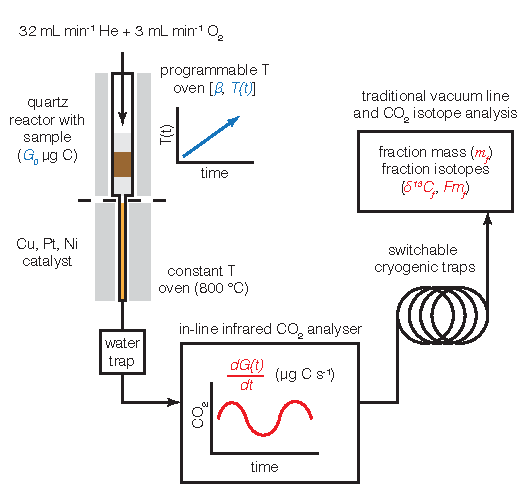
\includegraphics[]{Thesis_Figures/Ch3Fig1}}
	\caption[Schematic of the RPO instrumental setup]{Schematic of the RPO instrumental setup. User-defined inputs are printed in blue, while resulting observed measurements are printed in red (See Table \ref{Ch3Tab:1} for symbol definitions). }
	\label{Ch3Fig:1} 
\end{figure}

% Table 1
\begin{table}[p]
	\caption[List of mathematical symbols used throughout this study]{List of mathematical symbols used throughout this study.}
	\centering
		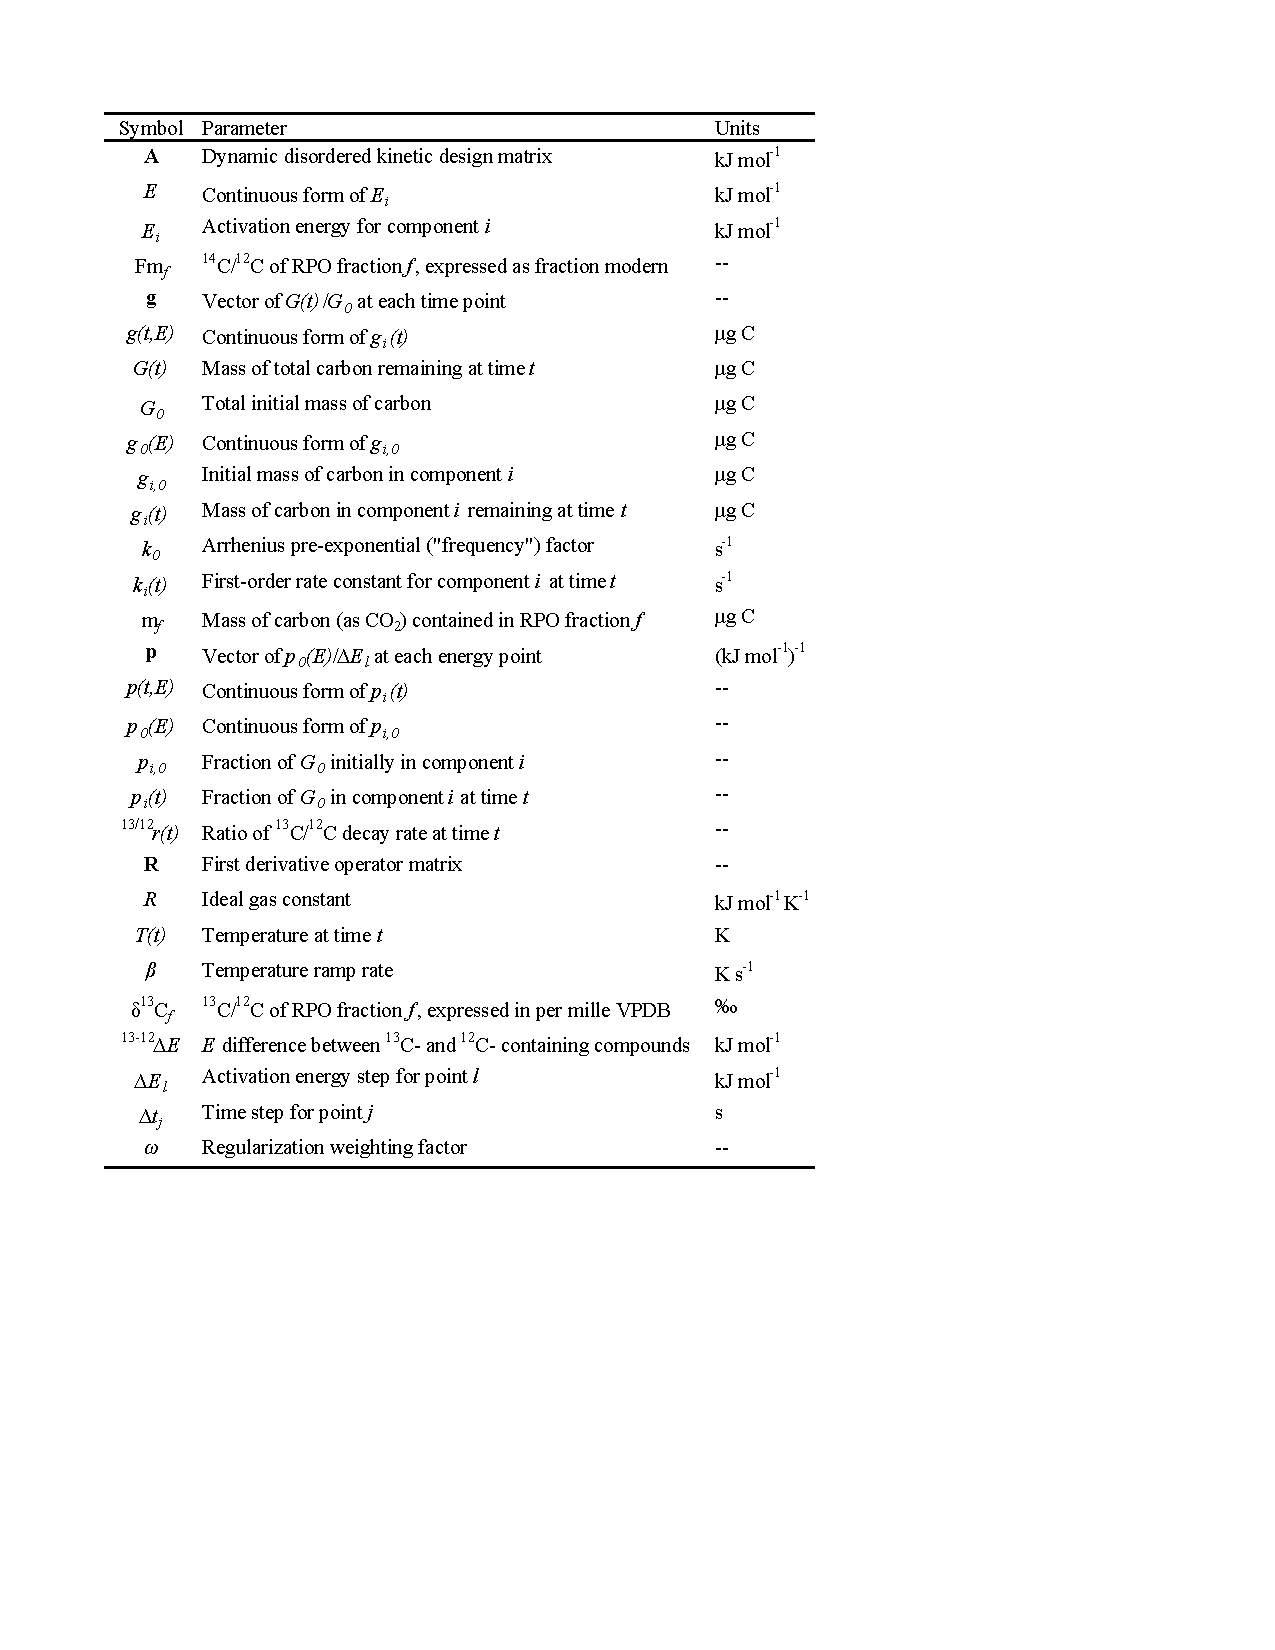
\includegraphics{Thesis_Tables/Ch3Tab1}
	\label{Ch3Tab:1} 
\end{table}

\subsection{Isotope measurement, blank correction, and data processing}

After recombustion at \SI{525}{\celsius} for 1 hour to remove trace contaminant gases, isotope composition of \ce{CO2} contained in each RPO fraction was analyzed following standard procedures \citep{McNichol:1994ty,Pearson:1998vy}, where \ce{^{13}C} content is expressed in \ce{\delta^{13}C} per mille (\si{permil}) notation relative to Vienna Pee Dee Belemnite (VPDB) and \ce{^{14}C} content is expressed in fraction modern (Fm) notation following \citet{Stuiver:1977uh}. We note that Fm as reported here is identical to the "\ce{^{14}a_{N}}" notation of \citet{Mook:1999vf} as well as the "\ce{F^{14}C}" notation of \citet{Reimer:2004th}. RPO fraction masses, \ce{\delta^{13}C} values, and Fm values were corrected for blank carbon contribution, and \ce{\delta^{13}C} was additionally corrected to ensure \ce{^{13}C} mass balance as incomplete oxidation to \ce{CO2} has been shown to exhibit a small fractionation effect \citep{Hemingway:2016rc}. Analytical uncertainty was propagated throughout all corrections.

All calculations contained herein were performed using the open-source 'rampedpyrox' package for Python v.3.5 as described in \citet{Hemingway:bA3-kvLz}.

\section{Results}

RPO fraction temperature ranges, \ce{CO2} masses, \ce{\delta^{13}C}, and Fm are reported in Tables \ref{Ch3Tab:2}--\ref{Ch3Tab:4} along with independently measured bulk isotope composition for each sample. The resulting Narayani PB-60 thermogram can be described as a bimodal distribution with peaks at \SI{365}{\celsius} and \SI{662}{\celsius}, similar to that observed previously when analyzed in pyrolysis mode \citep[Figure \ref{Ch3Fig:2}A;][]{Rosenheim:2012kh}. Corresponding RPO fraction Fm values decrease monotonically between \SI{150}{\celsius} and \SI{725}{\celsius} from \num{0.891 \pm 0.004} (fraction 1) to \num{0.014 \pm 0.002} (fraction 8), followed by a small yet statistically significant increase to \num{0.042 \pm 0.002} in the final fraction. \ce{\delta^{13}C} values display the opposite trend, rising from \SI{-29.5 \pm 0.2}{\permil.VPDB} (fraction 1) to \SI{-21.8 \pm 0.2}{\permil.VPDB} (fraction 8) followed by a slight decrease to \SI{-23.5 \pm 0.2}{\permil.VPDB}. 

% Table 2
\begin{sidewaystable}[p]
	\caption[Narayani PB-60 RPO results]{Narayani PB-60 measured RPO temperature ranges, \ce{CO2} masses, \ce{\delta^{13}C}, Fm, and modeled $E$ values for each fraction. Also included are mass-weighted averages [$\Sigma(1-9)$] and independently measured bulk isotope values.}
	\centering
		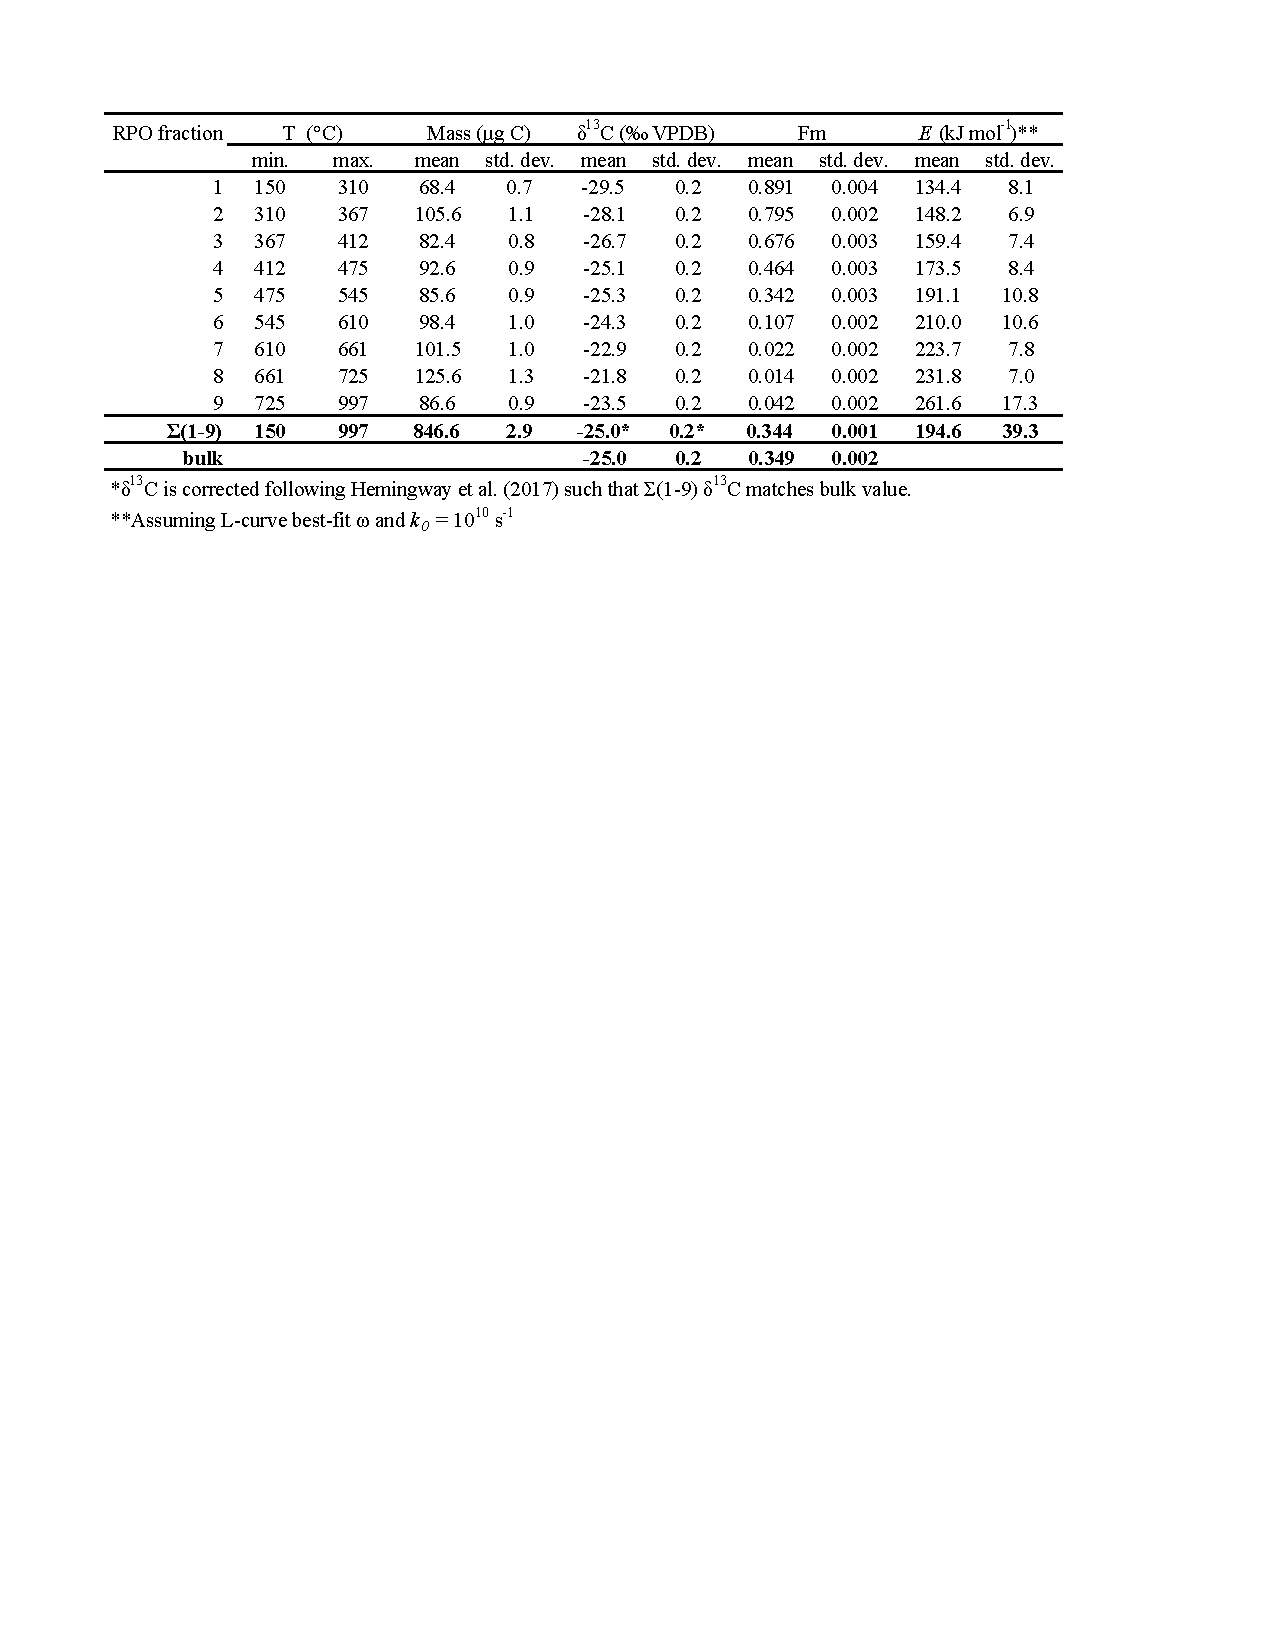
\includegraphics{Thesis_Tables/Ch3Tab2}
	\label{Ch3Tab:2} 
\end{sidewaystable}

% Table 3
\begin{sidewaystable}[p]
	\caption[JGOFS MC-1 RPO results]{JGOFS MC-1 measured RPO temperature ranges, \ce{CO2} masses, \ce{\delta^{13}C}, and modeled $E$ values for each fraction. Also included are mass-weighted averages [$\Sigma(1-5)$] and the independently measured bulk \ce{\delta^{13}C} value.}
	\centering
		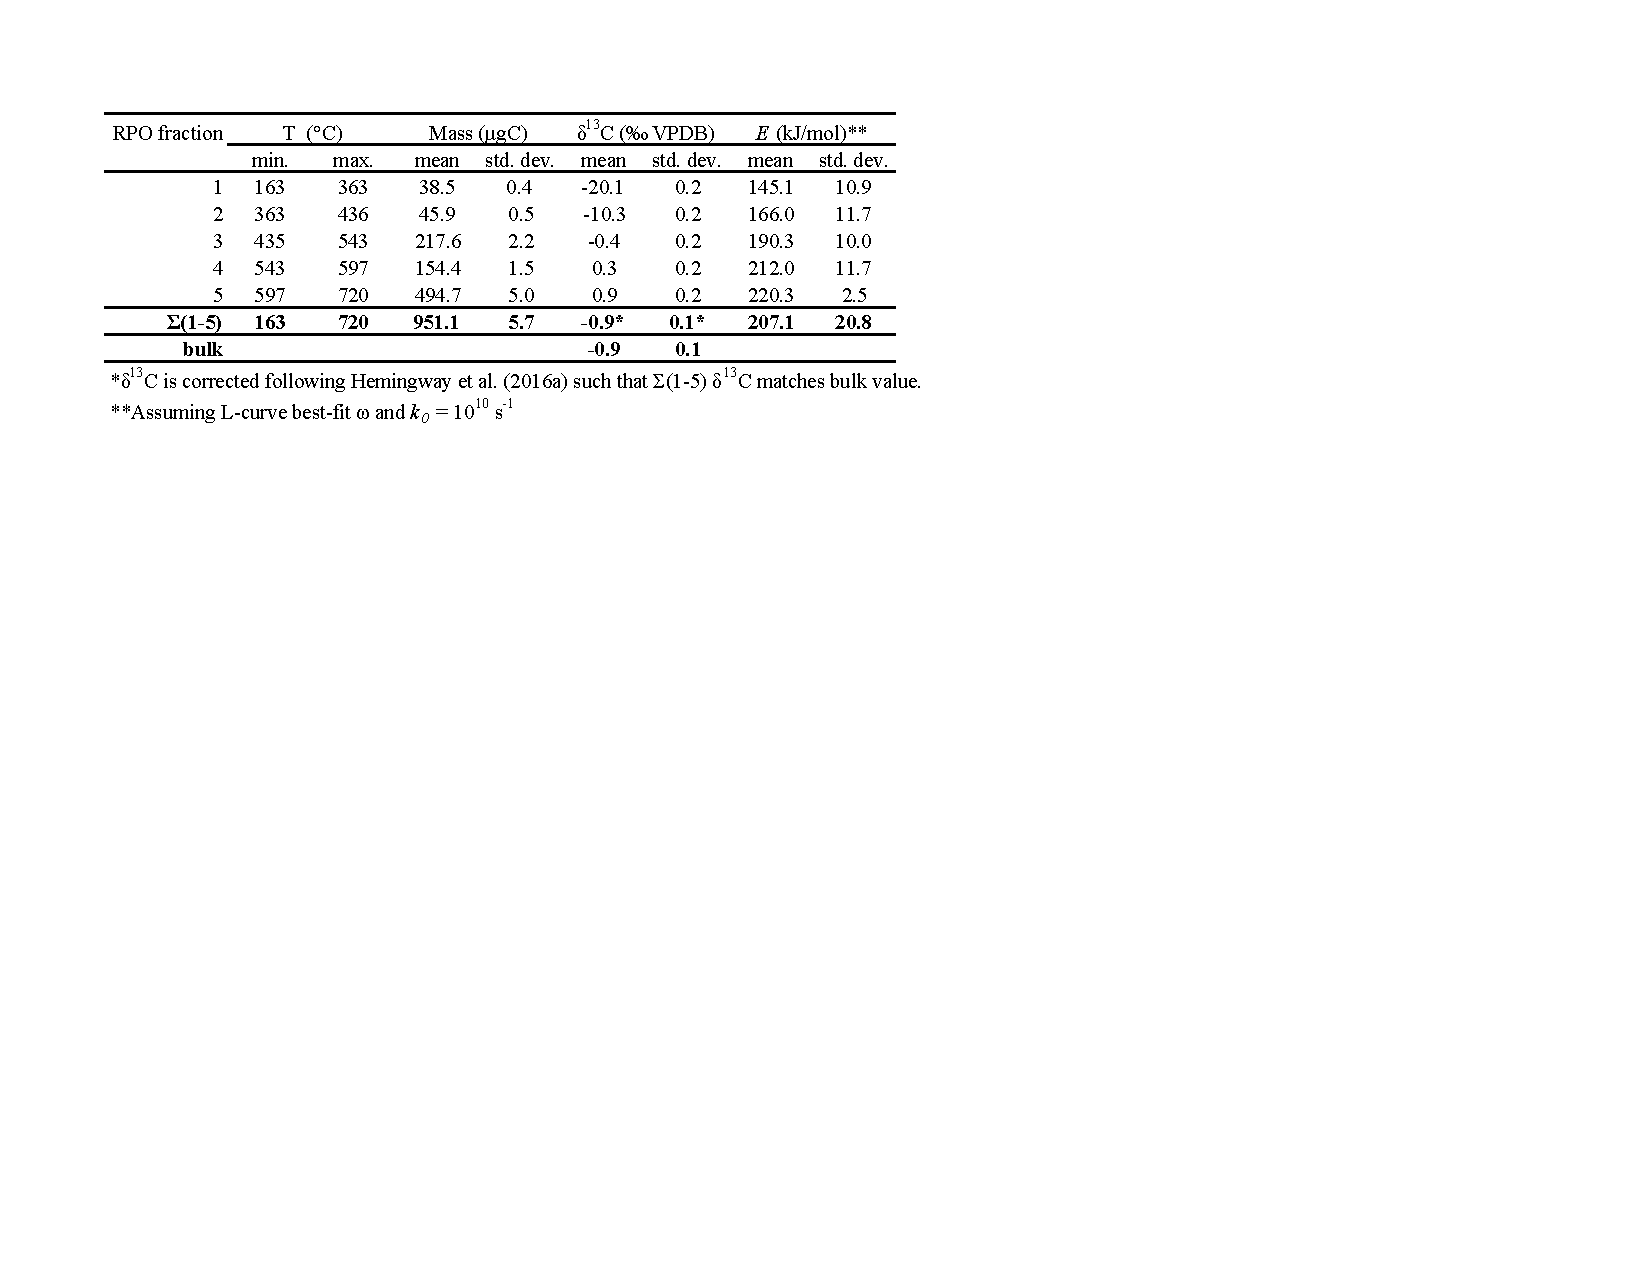
\includegraphics{Thesis_Tables/Ch3Tab3}
	\label{Ch3Tab:3} 
\end{sidewaystable}

% Table 4
\begin{sidewaystable}[p]
	\caption[Pololu 4169 RPO results]{Pololu 4169 measured RPO temperature ranges, \ce{CO2} masses, \ce{\delta^{13}C}, Fm, and modeled $E$ values for each fraction. Also included are mass-weighted averages [$\Sigma(1-5)$] and independently measured bulk isotope values.}
	\centering
		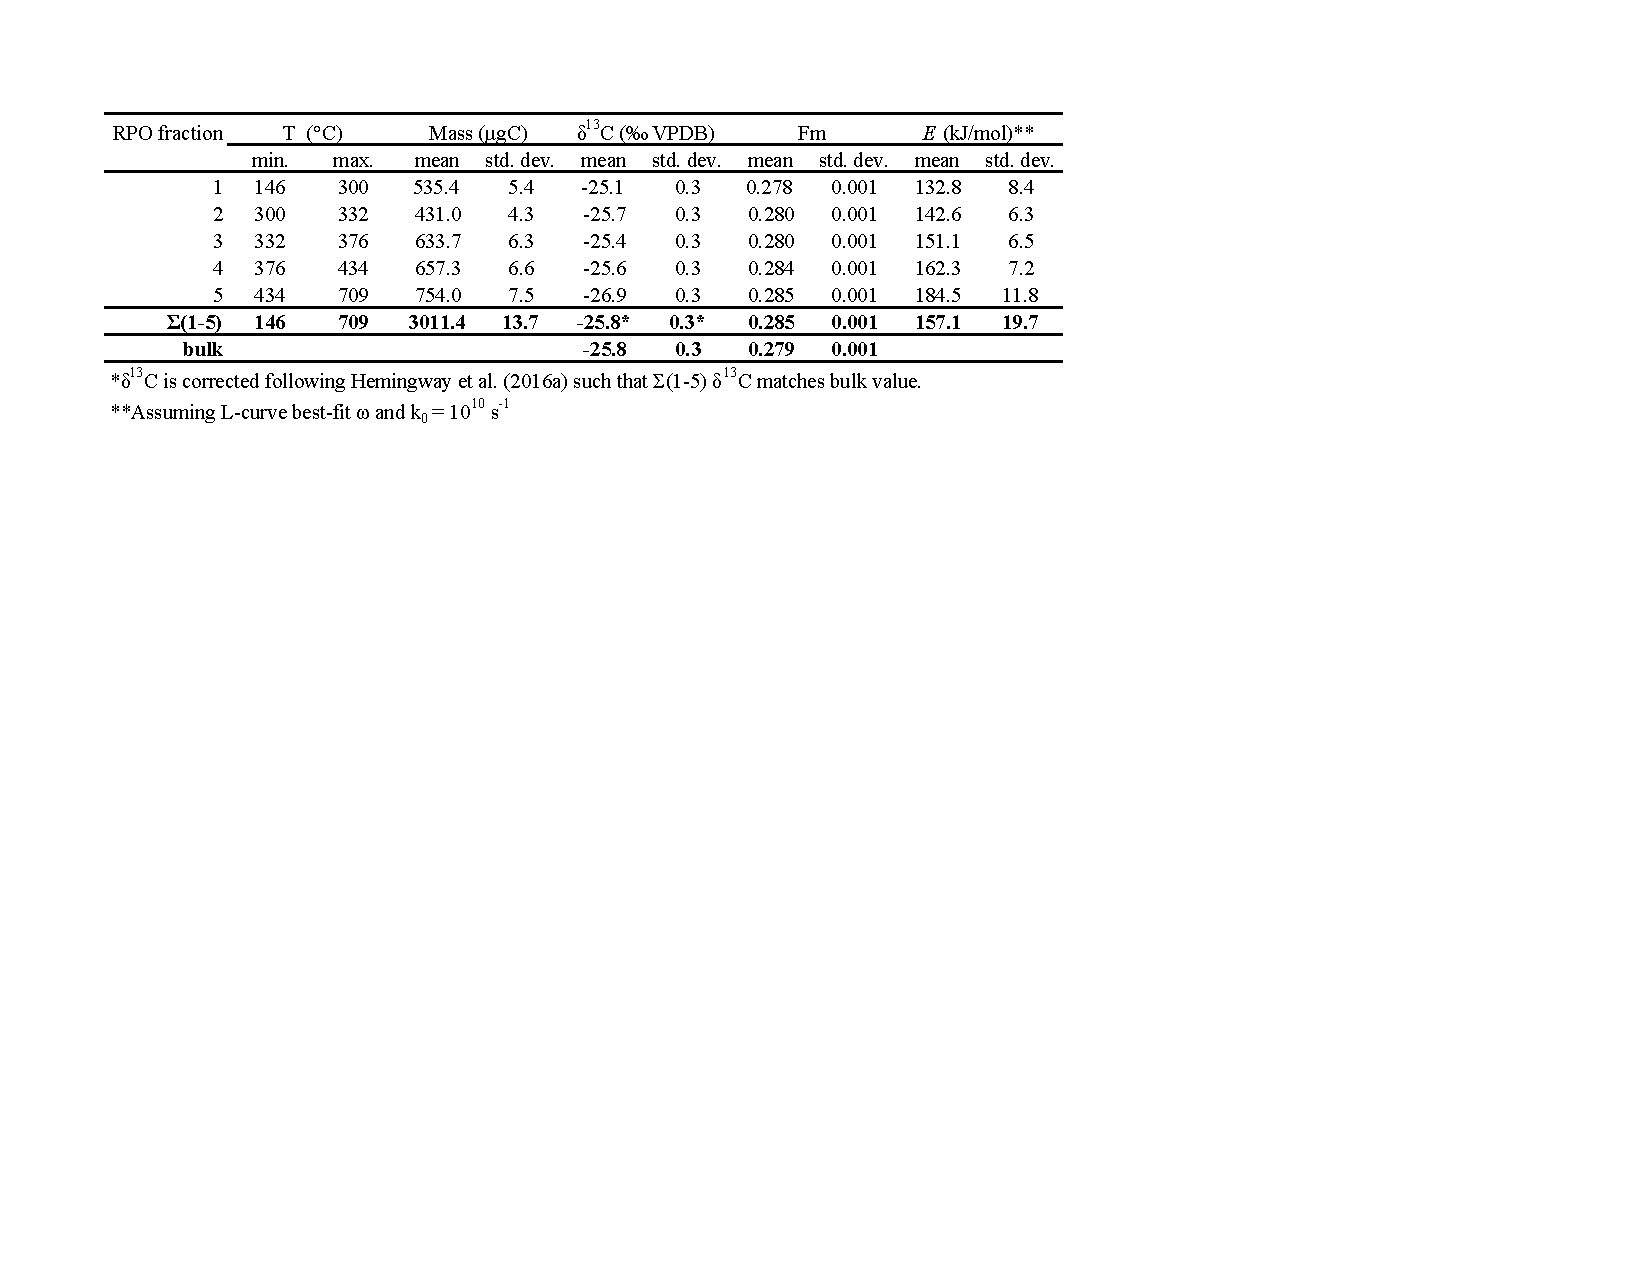
\includegraphics{Thesis_Tables/Ch3Tab4}
	\label{Ch3Tab:4} 
\end{sidewaystable}

In contrast, the JGOFS MC-1 thermogram is dominated by a single peak with a maximum decay rate at \SI{652}{\celsius} (Figure \ref{Ch3Fig:2}B). This is within the range of previously observed carbonate decomposition temperatures \citep{Plante:2013tu}, consistent with the fact that \SI{\approx 95}{\%} of the carbon in this sample is present as calcite \citep{Sayles:2001ua}. While Fm was not measured, \ce{\delta^{13}C} values increase drastically throughout the experiment from \SI{-20.1 \pm 0.2}{\permil.VPDB} (fraction 1) to \SI{0.9 \pm 0.2}{\permil.VPDB} (fraction 5). Lastly, carbon contained in Pololu 4169 exhibits the lowest degradation temperatures of all samples studied, with a maximum decay rate at \SI{348}{\celsius} and \SI{<0.5}{\%} of initial carbon remaining unreacted at \SI{600}{\celsius} (Figure \ref{Ch3Fig:2}C). Fm values are remarkably stable across RPO fractions, ranging from \num{0.278 \pm 0.001} (fraction 1) to \num{0.285 \pm 0.001} (fraction 5). Despite this, \ce{\delta^{13}C} values display a significant decrease with increasing temperature, ranging from \SI{-25.1 \pm 0.3}{\permil.VPDB} (fraction 1) to \SI{-26.9 \pm 0.3}{\permil.VPDB} (fraction 5). 

% Figure 2
\begin{figure}[p]
	\makebox[\textwidth][c]{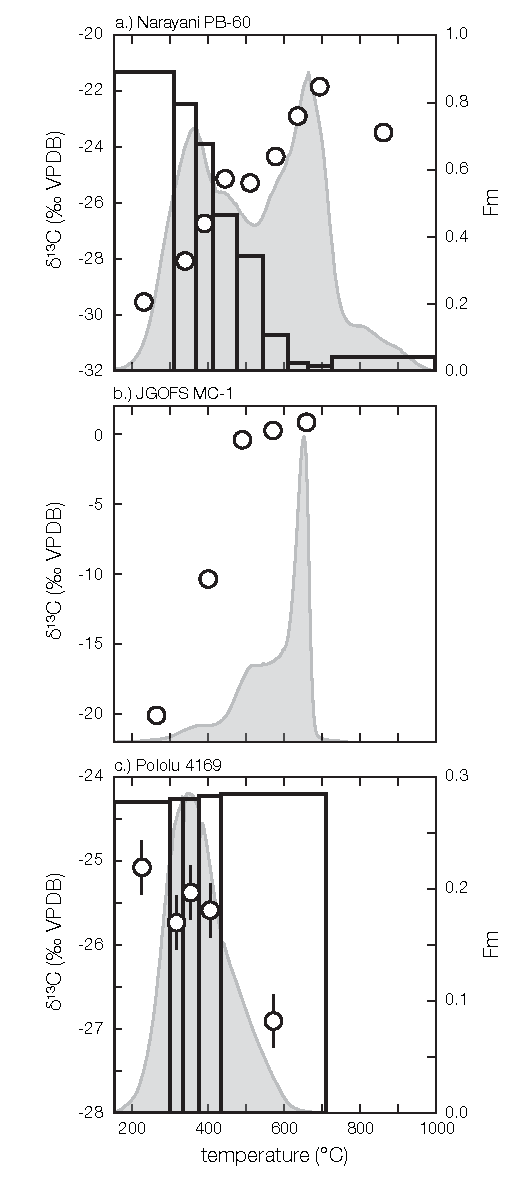
\includegraphics[]{Thesis_Figures/Ch3Fig2}}
	\caption[RPO thermograms, \ce{\delta^{13}C}, and Fm values for all samples]{RPO mass-normalized thermograms (gray shaded region, unitless), \ce{\delta^{13}C} values (white circles, left axis), and Fm values (transparent bars, right axis) for \textit{(A)} Narayani PB-60, \textit{(B)} JGOFS MC-1 (Fm not measured), and \textit{(C)} Pololu 4169. Width of Fm bars corresponds to the temperature range of collection for each RPO fraction. Where visible, \ce{\delta^{13}C} error bars represent propagated analytical uncertainty (Fm uncertainty not visible).}
	\label{Ch3Fig:2} 
\end{figure}

To test if thermogram shapes depend on initial carbon mass ($G_0$), we reanalyzed Nayarani PB-60 and JGOFS MC-1 for various values of $G_0$ while holding all other experimental conditions constant (\textit{i.e.} $\beta = 5$ \si{\celsius.min^{-1}}). Narayani PB-60 thermograms scale linearly with $G_0$ throughout the experiment, with maximum decay rates ranging from \SI{\approx 0.06}{\micro g.C.s^{-1}} ($G_0 = 268$ \si{\micro g.C}) to \SI{\approx 0.20}{\micro g.C.s^{-1}} ($G_0 = 828$ \si{\micro g.C}; Figure \ref{Ch3Fig:3}A). $G_0$ has no apparent effect on elution temperature for this sample, with maximum decay rates observed at \SI{662.0 \pm 0.8}{\celsius} for all values of $G_0$. Similarly, JGOFS MC-1 decay rates scale positively with $G_0$, with a maximum decay rate ranging from \SI{\approx 0.10}{\micro g.C.s^{-1}} ($G_0 = 98$ \si{\micro g.C}) to \SI{\approx 0.88}{\micro g.C.s^{-1}} ($G_0 = 951$ \si{\micro g.C}; Figure \ref{Ch3Fig:3}B). However, unlike Narayani PB-60, the temperature at which maximum decay rates are observed increases with $G_0$ from \SI{620.5}{\celsius} ($G_0 = 98$ \si{\micro g.C}) to \SI{652.2}{\celsius} ($G_0 = 951$ \si{\micro g.C}).

Lastly, we analyzed Narayani PB-60 at multiple ramp rates ($\beta$ = \SIlist{2;5;10}{\celsius.min^{-1}}) while holding $G_0$ constant. Here we normalize thermograms by initial mass and ramp rate in order to accurately compare between experimental conditions, resulting in plots of fractional carbon loss per \si{\celsius} (Figure \ref{Ch3Fig:3}C). Results indicate a consistent shift toward higher elution temperatures for higher ramp rates, as predicted by parallel first-order kinetics \citep{Braun:1987vf,Miura:1995uo,Miura:1998jf}. For example, the temperature at which the maximum decay rate is reached increases from \SI{621.2}{\celsius} when $\beta = 2$ \si{\celsius.min^{-1}} to \SI{688.5}{\celsius} when $\beta = 10$ \si{\celsius.min^{-1}}. This temperature increase is accompanied by a corresponding decrease in decay rate, with maximum values dropping from \SI{3.1e-3}{\celsius^{-1}} ($\beta = 2$ \si{\celsius.min^{-1}}) to \SI{2.7e-3}{\celsius^{-1}} ($\beta = 10$ \si{\celsius.min^{-1}}).

% Figure 3
\begin{figure}[p]
	\makebox[\textwidth][c]{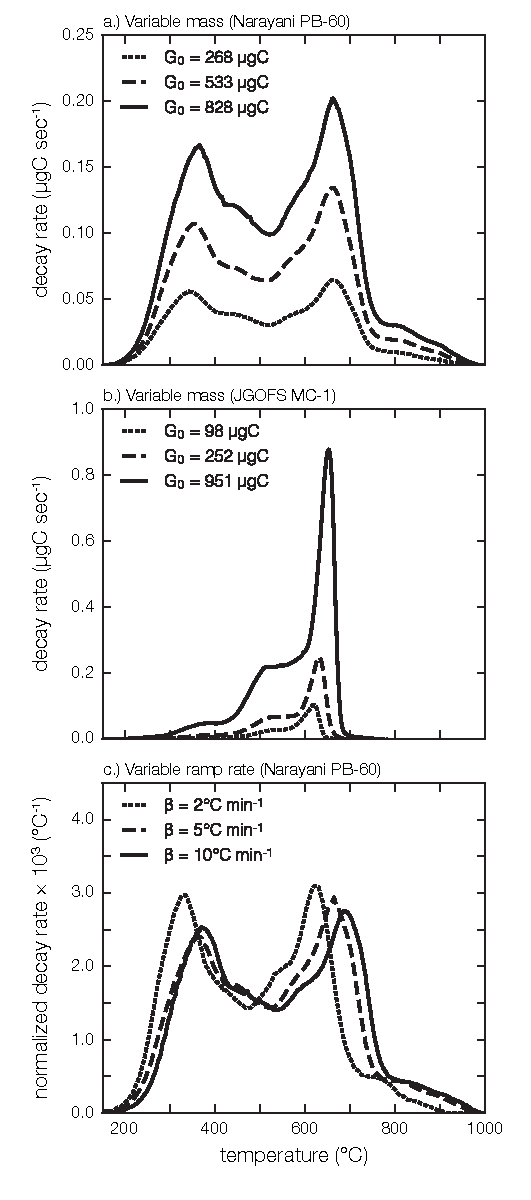
\includegraphics[]{Thesis_Figures/Ch3Fig3}}
	\caption[The effects of initial mass ($G_{0}$) and ramp-rate ($\beta$) on RPO thermograms]{Testing the effects of initial mass ($G_{0}$) and ramp-rate ($\beta$) on RPO thermograms: \textit{(A)} Narayani PB-60 and \textit{(B)} JGOFS MC-1 analyzed for multiple $G_{0}$ values,  \textit{(C)} Narayani PB-60 analyzed for multiple $\beta$ values. Decay rates in panel \textit{(C)} are normalized by $G_{0}$ and $\beta$ in order to properly compare between each analysis.}
	\label{Ch3Fig:3} 
\end{figure}

\section{Discussion}

To properly interpret RPO thermograms as a function of OC chemical composition, and to relate these results with corresponding \ce{\delta^{13}C} and Fm values, remineralization kinetics during thermal degradation must be fully constrained. The distributed activation energy model (DAEM) is a promising method to do so, as it has long been utilized to describe the non-isothermal decay of complex carbon mixtures such as biomass \citep[\textit{e.g.}][]{Bradbury:1979to,White:2011iz} and fossil fuel precursor OC \citep[\textit{e.g.}][]{Burnham:1987ut,Braun:1987vf,Burnham:1999ec,Cramer:2004tg,Dieckmann:2005dw} during thermogravimetric analysis. Here we derive the DAEM  by first considering the case where OC is separated into a finite set of discrete components with unique activation energy values. We then generalize this description to allow for a continuous distribution of OC quality, as has been done previously \citep[see][for review]{Burnham:1999ec}. Finally, following \citet{Forney:2012dr,Forney:2012hz}, we describe an inverse method to determine the regularized solution of the ill-posed DAEM, and compare resulting reaction energetics with RPO fraction \ce{\delta^{13}C} and Fm values.

\subsection{Mathematical derivation}

\subsubsection{Discrete DAEM}

First, we consider the case where OC is described by a finite set of discrete components associated with unique activation energy values. During OC remineralization, the decay rate of carbon contained in a particular component $i$ is often described as as a first-order process with respect to the mass of carbon remaining in component $i$ at any time $t$, $g_{i}(t)$ \citep{Berner:1980ux,Braun:1987vf}:
%
% Equation 1
\begin{equation}\label{Ch3Eq:1}
	\frac{dg_{i}(t)}{dt} = - k_{i}(t) g_{i}(t)
\end{equation}
%
where $k_{i}(t)$ is the dynamic first-order rate coefficient associated with component $i$ at time $t$. Although OC decay in the environment can additionally depend on oxidant concentration, we omit this dependency here since \ce{O2} is provided in excess in our experimental setup. In contrast to the "multi-G" and "reactive continuum" models that are often used to describe environmental OC degradation rates \citep{Westrich:1984uj,Boudreau:1991wf,Forney:2012dr,Forney:2012hz}, here we explicitly allow $k_{i}(t)$ to vary with time. Because rate coefficients are related to temperature and activation energy, $k_{i}(t)$ can be determined as a function of $E$ following the Arrhenius equation so long as temperature is known at each time point:
%
% Equation 2
\begin{equation}\label{Ch3Eq:2}
	k_{i}(t) = k_{0} \exp \left[ - \frac{E_{i}}{RT(t)} \right]
\end{equation}
%
where $k_0$ is the empirically derived Arrhenius pre-exponential ("frequency") factor, $R$ is the ideal gas constant, $E_{i}$ is the activation energy of carbon contained in component $i$, and $T(t)$ is the measured temperature of the system at time $t$. For non-isothermal systems, time-dependent (\textit{i.e.} dynamic) decay coefficients can therefore be described by the static property $E_{i}$ and the observed variable $T(t)$. Although $T(t)$ is related to $t$ by a constant ramp rate $\beta$ during RPO analysis, we leave this written as is to emphasize that the DAEM is valid for any measured time-temperature history. Substituting Equation \ref{Ch3Eq:2} for $k_{i}(t)$, first-order decay during a non-isothermal process at time $t$ can be written as:
%
% Equation 3
\begin{equation}\label{Ch3Eq:3}
	\frac{dg_{i}(t)}{dt} = - k_{0} \exp \left[ - \frac{E_{i}}{RT(t)} \right] g_{i}(t)
\end{equation}
%
The mass of carbon remaining in component $i$ at time $t$ is therefore determined by integrating Equation \ref{Ch3Eq:3} from an initial time, $t_{0} = 0$, to a final time $t$:
%
% Equation 4
\begin{equation}\label{Ch3Eq:4}
	g_{i}(t) = g_{i,0} \exp \left[ - k_{0} \int_{0}^{t} \exp \left\{ - \frac{E_{i}}{RT(t')} \right\} dt' \right]
\end{equation}
%
where $g_{i,0}$ is the initial mass of carbon contained in component $i$ and $t'$ is the change-of-variables substituted time variable ranging from $t_{0} = 0$ to $t$. Due to the integration of the Arrhenius equation from $t_{0} = 0$ to $t$, Equation \ref{Ch3Eq:4} states that $g_{i}(t)$ depends on the entire time-temperature history of the experiment. That is, $\frac{dg_{i}(t)}{dt}$ is governed by a balance between decreasing $g_{i}(t)$ as OC is remineralized and increasing $k_{i}(t)$ with increasing $T(t)$ as the experiment progresses. This balance should result in a predictable shift in RPO thermograms toward higher elution temperatures with increasing $\beta$, as is observed \citep[Figure \ref{Ch3Fig:3}C;][]{Braun:1987vf,Miura:1995uo,Miura:1998jf}.

Furthermore, following the multi-G model of \citet{Westrich:1984uj}, any environmental sample containing a complex OC mixture can be described as a superposition of a finite set of $n$ components, each decaying according to a unique $k_{i}(t)$ and thus corresponding to a unique $E_{i}$ value. The total carbon mass remaining at $t$, $G(t)$, is therefore the sum of the mass remaining in each component $i = 1,2,\dots,n$ at that time:
%
% Equation 5
\begin{equation}\label{Ch3Eq:5}
	\begin{split}
		G(t) & = \sum_{i=1}^{n} g_{i}(t) \\
		& =  G_{0} \sum_{i=1}^{n} p_{i,0} \exp \left[ - k_{0} \int_{0}^{t} \exp \left\{ - \frac{E_{i}}{RT(t')} \right\} dt' \right]
	\end{split}
\end{equation}
%
where $G_{0}$ is the initial OC mass present in the entire sample, defined as the sum of initial mass contained in each component:
%
% Equation 6
\begin{equation}\label{Ch3Eq:6}
	G_{0} = \sum_{i=1}^{n} g_{i,0}
\end{equation}
%
and $p_{i,0}$ is the fraction of total carbon initially contained in component $i$:
%
% Equation 7
\begin{equation}\label{Ch3Eq:7}
	p_{i,0} = \frac{g_{i,0}}{G_{0}}
\end{equation}
%
such that $\sum_{i=1}^{n} p_{i,0} \equiv 1.0$. The fraction of OC initially present within each component can therefore be determined by fitting Equation \ref{Ch3Eq:5} to the observed $G(t)$ profile measured by the RPO instrument. While informative, this discrete description of the DAEM suffers from two major limitations: \textit{(i)} $n$ must be set \textit{a priori} or determined empirically \citep{Boudreau:1991wf} and \textit{(ii)} any noise recorded in the data will result in large uncertainty in best-fit $p_{i,0}$ and $E_{i}$ values \citep{Forney:2012hz}. To circumvent these issues, a more general description of non-isothermal first-order decay can be derived that does not assume a finite set of components with unique $E_{i}$, but rather allows $E$ to vary continuously \citep{Burnham:1987ut,Burnham:1999ec,Cramer:2004tg}.

\subsubsection{Continuous DAEM}

In this continuous model, the mass of carbon remaining at time $t$ that is associated with any activation energy value $E$, $g(t, E)$, can be determined by substituting $g(t,E)$ for $g_{i}(t)$ and $E$ for $E_{i}$ in Equation \ref{Ch3Eq:4}:
%
% Equation 8
\begin{equation}\label{Ch3Eq:8}
	g(t, E) = g_{0}(E) \exp \left[ - k_{0} \int_{0}^{t} \exp \left\{ - \frac{E}{RT(t')} \right\} dt' \right]
\end{equation}
%
where $g_{0}(E)$ is the initial mass of carbon associated with activation energy value $E$. The total carbon mass remaining at time $t$, $G(t)$, can now be defined by replacing the summation over components $i = 1,2,\dots,n$ in Equation \ref{Ch3Eq:5} by an integral over all possible (\textit{i.e.} non-negative) values of $E$:
%
% Equation 9
\begin{equation}\label{Ch3Eq:9}
	\begin{split}
	G(t) & = G_{0} \int_{0}^{\infty} p_{0}(E) \\
	& \qquad\qquad \exp \left[ - k_{0} \int_{0}^{t} \exp \left\{ - \frac{E}{RT(t')} \right\} dt' \right] dE
	\end{split}
\end{equation}
%
where $p_{0}(E) dE$ is now the fraction of total carbon initially associated with the infinitesimal range of activation energy values about $E$ such that:
%
% Equation 10
\begin{equation}\label{Ch3Eq:10}
    \int_{0}^{\infty} p_{0}(E) dE  \equiv 1
\end{equation}
%
That is, the distribution of $p_{0}(E)$ over all values of $E$ describes the initial probability density function (pdf) of activation energy that will lead to the observed OC decay rates when a sample is analyzed in the RPO instrument. Unlike measured thermograms, $p_{0}(E)$ is not a function of experimental conditions such as ramp rate -- rather, it is an intrinsic property of the physical-chemical bonding environment within a particular sample. As RPO analysis proceeds, this pdf must evolve with time to reflect the fact that some carbon has been remineralized to \ce{CO2}. Therefore, at any time $t$ the remaining fraction of total OC initially present in the sample that is associated with any activation energy value, $p(t, E) dE$, is calculated as $p_{0}(E)dE$ multiplied by a double exponential decay term analogous to Equation \ref{Ch3Eq:8}:
%
% Equation 11
\begin{equation}\label{Ch3Eq:11}
	p(t,E) dE = p_{0}(E) \exp \left[ - k_{0} \int_{0}^{t} \exp \left\{ - \frac{E}{RT(t')} \right\} dt' \right] dE
\end{equation}
%
Equation \ref{Ch3Eq:11} implies that the carbon initially remineralized to \ce{CO2} must be associated with the lowest values of $E$, as low $E$ will lead to a double exponential term that approaches zero most rapidly. Put differently, OC that is described by higher $E$ values will resist remineralization until more time has passed and, therefore, higher temperatures have been reached -- \textit{i.e.} it is more thermally recalcitrant.

\subsection{Verification of parallel first-order kinetics}

Because the DAEM is a specific case of \textit{n}-order non-isothermal kinetic models \citep{Braun:1987vf,White:2011iz}, we must verify that carbon degradation in the RPO instrument behaves according to a superposition of parallel first-order reactions (with respect to OC concentration) rather than higher-order processes. Differentiating Equation \ref{Ch3Eq:9} with respect to time, the total rate of carbon remineralization at any time $t$ is given by the equation:
%
% Equation 12
\begin{equation} \label{Ch3Eq:12}
	\begin{split}
	\frac{dG(t)}{dt}  & = - G_{0} \int_{0}^{\infty} p_{0}(E) k_{0} \exp \left[ - \frac{E}{RT(t)} \right] \\
		& \qquad\qquad \exp \left[ - k_{0} \int_{0}^{t} \exp \left\{ - \frac{E}{RT(t')} \right\} dt' \right] dE \\
	& = - G_{0} \int_{0}^{\infty} p(t, E) k_{0} \exp \left[ - \frac{E}{RT(t)} \right] dE \\
	\end{split}
\end{equation}
%
It can be seen that the DAEM describes $\frac{dG(t)}{dt}$ as a linear function of $G_{0}$ multiplied by an integral term that depends on $p(t,E)$ but is independent of $G_{0}$. In contrast, if carbon decomposition within the RPO instrument were to follow a higher-order process, the relationship between $\frac{dG(t)}{dt}$ and $G_{0}$ would be nonlinear and evolve as a function of time \citep[\textit{e.g.}][]{Follett:2014if}. Replacing the integral term in Equation \ref{Ch3Eq:12} by $m(t)$, the loss of carbon at time $t$ as predicted by the DAEM simplifies to:
%
% Equation 13
\begin{equation} \label{Ch3Eq:13}
	\frac{dG(t)}{dt} = - G_{0} m(t)
\end{equation}
%
Therefore, similar to the isothermal case described in \citet{Follett:2014if}, a superposition of parallel first-order decay reactions will result in a linear relationship between $\frac{dG(t)}{dt}$ and $G_{0}$ with a zero intercept and a time-dependent slope equal to:
%
% Equation 14
\begin{equation}\label{Ch3Eq:14}
 	m(t) = \int_{0}^{\infty} p(t, E) k_{0} \exp \left[ - \frac{E}{RT(t)} \right] dE
\end{equation}
%
where $m(t)$ can be interpreted as the $G_{0}$-normalized decay rate at time $t$. We verify that OC remineralization within the RPO instrument follows parallel first-order kinetics by assessing the linearity between $\frac{dG(t)}{dt}$ and $G_{0}$ at any time $t$ across a range of $G_{0}$ values using Narayani PB-60 a test sample (Figure \ref{Ch3Fig:3}A). We chose Narayani PB-60 because it exhibits the widest range of decomposition temperatures of any sample analyzed here (Figure \ref{Ch3Fig:2}). For 4 arbitrarily chosen time points, it can be seen that this relationship is linear with an ordinary least squares $R^{2} \geq 0.999$ (Figure \ref{Ch3Fig:4}A), resulting in identical $G_{0}$-normalized thermograms within analytical uncertainty (Figure \ref{Ch3Fig:4}B). Therefore, the decay of complex OC mixtures contained in decarbonated samples during RPO analysis can indeed be accurately described by a superposition of parallel first-order reactions.

% Figure 4
\begin{figure}[p]
	\makebox[\textwidth][c]{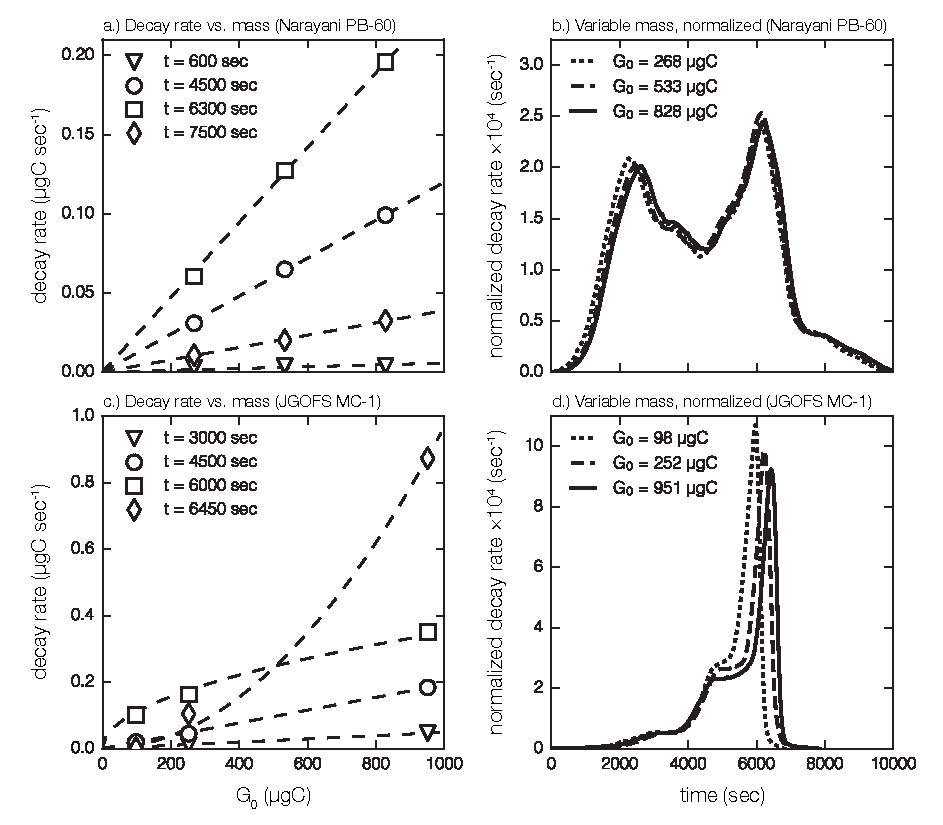
\includegraphics[]{Thesis_Figures/Ch3Fig4}}
	\caption[Assessment of first-order kinetics]{First-order kinetic assessment: \textit{(A)} decay rate vs. $G_{0}$ relationships at four arbitrarily chosen time points for Narayani PB-60, including best-fit regressions (dashed lines); \textit{(B)} mass-normalized decay rates for each analysis used in \textit{(A)}; \textit{(C)} decay rate vs. $G_{0}$ relationships at four arbitrarily chosen time points for JGOFS MC-1, including best-fit regressions (dashed lines); and \textit{(D)} mass-normalized decay rates for each analysis used in \textit{(C)}. Linear relationships and nearly identical normalized decay rates in panels \textit{(A)--(B)} confirm the first-order nature of OC decay, while non-linear relationships and a shifting carbonate peak in panels \textit{(C)--(D)} indicate non-first-order \ce{CaCO3} decay kinetics.}
	\label{Ch3Fig:4} 
\end{figure}

\subsubsection{A note of caution for carbonates}\label{Ch3Sec:3521}

While most RPO studies to date have focused on OC analysis by acidifying to remove carbonates \citep[\textit{e.g.}][]{Rosenheim:2008ed,Rosenheim:2012kh,Rosenheim:2013dka,Schreiner:2014jr,Bianchi:2015jr}, it has recently been argued that acid hydrolysis and/or dissolution of short range order minerals during acid treatment can alter the OC chemical bonding environment and therefore affect thermal stability \citep{Plante:2013tu}. Analyzing raw samples without acid treatment can circumvent these issues, however the effect of carbonates on decay kinetics has not yet been considered. To test if carbonate-rich samples follow parallel first-order kinetics, we similarly analyzed JGOFS MC-1 for a range of $G_{0}$ values (Figure \ref{Ch3Fig:3}B). Prior to $t \approx 4500$ s, when \ce{\delta^{13}C} values of eluted \ce{CO2} indicate a predominantly OC source (Figure \ref{Ch3Fig:2}B), $\frac{dG(t)}{dt}$ can be accurately described as a linear function of $G_{0}$ ($R^{2} \geq 0.999$). However, as carbonate begins to decompose above $t \approx 4500$ s, the relationship between $\frac{dG(t)}{dt}$ and $G_{0}$ becomes highly nonlinear -- that is, the resulting carbonate peak shifts toward higher $t$ with increasing $G_{0}$ (Figure \ref{Ch3Fig:4}C--D). 

To investigate if non-first-order decomposition is an intrinsic property of \ce{CaCO3} or if this is due to interactions with other materials within the sample (so-called "matrix effects"), we additionally analyzed a purified Icelandic spar \ce{CaCO3} standard at multiple masses ($G_{0}$ = \SIlist{258;492;1014}{\micro g.C}, $\beta$ = \SI{5}{\celsius.min^{-1}}). Results indicate that purified carbonate, unlike JGOFS MC-1, does follow first-order kinetics, with a maximum decomposition rate occurring at \SI{700 \pm 6}{\celsius} independent of $G_{0}$ (not shown). Interaction with reduced organic carbon, corresponding hetero-atoms (\textit{e.g.} N, P, S), or trace metals contained within the sample matrix are therefore the likely cause of non-first-order \ce{CaCO3} decomposition when analyzing environmental samples. Thus, while avoiding the issues of acid treatment, the analysis of carbonate-containing samples will result in thermograms that cannot be accurately described by the DAEM presented here, and is not recommended when using the RPO instrument to determine reaction energetics.


\subsection{Solving for $p_{0}(E)$ using an inverse method}

Following \citet{Forney:2012dr,Forney:2012hz}, we present a method to invert the DAEM and solve for the pdf of $E$ subject to a non-negativity constraint. In contrast to previous DAEM solutions \citep{Lakshmanan:1994vs,Cai:2007hh,deCaprariis:2012jk}, this approach does not require an \textit{a priori} assumption about the parametric form of $p_{0}(E)$. Additionally, because inverse methods are ill-posed and thus highly sensitive to noise, we "smooth" the solution using a Tikhonov regularization to remove this sensitivity \citep{Tikhonov:1977ui,Hansen:1994uc}. To numerically calculate $p_{0}(E)$, we discretize the continuous variable $t$ over the time course of the experiment into a vector $\mathbf{t}$ containing $n_{t}$ nodes, $t_{j}$, such that:
%
% Equation 15
\begin{equation}\label{Ch3Eq:15}
	\Delta t_{j} = \frac{1}{2} \left(t_{j} - t_{j-1} \right) + \frac{1}{2} \left(t_{j+1} - t_{j} \right)
\end{equation}
%
For generality, and because the DAEM is frequently applied over geologic timescales with non-uniformly distributed time measurements, Equation \ref{Ch3Eq:15} does not require a uniform time step (\textit{i.e.} it is possible that $\Delta t_{j} \neq \Delta t_{i \neq j}$). Similarly, we generate a vector $\mathbf{E}$ over the range values considered for the model solution (typically \SIrange{50}{350}{kJ.mol^{-1}}) that contains $n_{E}$ nodes, $E_{l}$, such that:
%
% Equation 16
\begin{equation}\label{Ch3Eq:16}
	\Delta E_{l} = \frac{1}{2} \left(E_{l} - E_{l-1} \right) + \frac{1}{2} \left(E_{l+1} - E_{l} \right)
\end{equation}
%
It can be seen from Equation \ref{Ch3Eq:9} that the DAEM can be separated into two components: \textit{(i)} $p_{0}(E)$ and \textit{(ii)} a double exponential term that is independent of $p_{0}(E)$. This term, analogous to the Laplace transform for the isothermal reactive continuum model \citep{Forney:2012hz}, describes the fraction of carbon initially associated with an activation energy value $E$ that has decayed by time $t$. We therefore generate a matrix $\mathbf{A}$ describing the dynamic disordered kinetics of the system by calculating the value of this term for all combinations of $t_{j}$ and $E_{l}$:
%
% Equation 17
\begin{equation}\label{Ch3Eq:17}
	A_{j,l} = \exp \left\{ -\sum_{u=0}^{j} k_{0} \exp \left[ - \frac{E_{l}}{RT(t_{u})} \right] \Delta t_{u} \right\} \Delta E_{l}
\end{equation}
%
Finally, we integrate the measured RPO thermogram and interpolate the resulting fraction of total carbon remaining at each time point, $\frac{G(t)}{G_{0}}$, onto each discretized time point in $\mathbf{t}$ to generate a vector of fractional carbon remaining, $\mathbf{g}$. The DAEM can thus be written in matrix form as:
%
% Equation 18
\begin{equation}\label{Ch3Eq:18}
	\mathbf{g} = \mathbf{A} \cdot \mathbf{p}
\end{equation}
%
where $\mathbf{p}$ is a discretized vector of $p_{0}(E)$ with length $n_{l}$ such that each component $p_{l}$ is equal to:
%
% Equation 19
\begin{equation}\label{Ch3Eq:19}
	p_{l} = \frac{1}{\Delta E_{l}} \int_{ \frac{1}{2} \left(E_{l} + E_{l-1} \right)}^{\frac{1}{2} \left(E_{l} + E_{l+1} \right)} p_{0}(E) dE
\end{equation}
%
While $\mathbf{p}$ can be calculated directly by multiplying $\mathbf{g}$ by the computed inverse of $\mathbf{A}$, it is possible that this will result in negative values of $p_{l}$ if $\mathbf{g}$ contains noisy data \citep{Forney:2012hz}. However, because $p_{l}$ represents a probability, it cannot be negative by definition. We therefore require the solution to be non-negative by solving the constrained least squares problem according to:
%
% Equation 20
\begin{equation}\label{Ch3Eq:20}
	\min_{\mathbf{p}} \| \mathbf{A} \cdot \mathbf{p} - \mathbf{g} \|^{2}
\end{equation}
%
where $\| \mathbf{x} \| \equiv \sqrt{ \sum x_{i}^{2}}$ is the vector norm and we require that $p_{l} \geq 0$. The resulting $\mathbf{p}$ vector is thus the non-regularized solution to the inverse DAEM.

\subsubsection{Choice of frequency factor}

In order to construct the $\mathbf{A}$ matrix and solve for $\mathbf{p}$, our method requires that the Arrhenius pre-exponential factor $k_{0}$ be prescribed \textit{a priori}. There exists significant discussion in the literature on the best choice of $k_{0}$, as multiple values of this parameter can describe laboratory results equally well but will result in drastically different predictions of OC degradation rates over geologic timescales \citep{Braun:1987vf,Burnham:1987ut,Lakshmanan:1991tr,Dieckmann:2005dw}. Furthermore, it has been argued that $k_{0}$ represents the variable change in entropy associated with the decay of specific organic compounds and should therefore be parameterized as a function of $E$ \citep[the so-called "kinetic compensation effect" or "KCE";][]{Tang:2000ua}. For example, a linear increase in $k_{0}$ with $E$ from \SI{\approx e8}{s.^{-1}} ($E$ = \SI{175}{kJ.mol^{-1}}) to \SI{\approx e26}{s^{-1}} ($E$ = \SI{400}{kJ.mol^{-1}}) has been utilized to better predict petroleum formation rates \citep{Dieckmann:2005dw}. To circumvent the issue of multiplicity, and to account for the KCE, \citet{Miura:1995uo} and \citet{Miura:1998jf} developed a method to estimate the best-fit $k_{0}$ for each value of $E$ by comparing the shift in elution temperatures when a sample is analyzed at multiple ramp rates (\textit{e.g.} Figure \ref{Ch3Fig:3}C). However, because this approach is based on large extrapolations in $\frac{1}{T}$ vs. $\frac{\beta}{T^{2}}$ space, it is highly sensitive to noise in temperature and $\beta$ measurements \citep{Burnham:1989vm}.

To select a best-fit $k_{0}$, here we calculate $\mathbf{A}$ and $\mathbf{p}$ for a range of $k_{0}$ values and determine the root mean squared error (RMSE) between measured $G(t)$ and that predicted by Equation \ref{Ch3Eq:20}. We include the KCE by calculating $k_{0}$ as a function of $E$ according to:
%
% Equation 21
\begin{equation}\label{Ch3Eq:21}
	\log_{10} k_{0} = (\text{KCE slope})E + (\text{KCE intercept})
\end{equation}
%
Resulting RMSE values using a range of KCE slope and intercept can be seen in Figure \ref{Ch3Fig:5} for Narayani PB-60 ($\beta$ = \SI{5}{\celsius.min^{-1}}, $E$ ranging from \SIrange{50}{350}{kJ.mol^{-1}}). By setting an "acceptable" cutoff of RMSE \num{\leq e-4}, it can be seen that there exist multiple KCE slope and intercept combinations that can equally fit the observed data. Additionally, we estimate the best-fit $k_{0}$ using a range of ramp rates ($\beta$ = \SIlist{2;5;10}{\celsius.min^{-1}}) following the method of \citet{Miura:1998jf} (Figure \ref{Ch3Fig:5}, white circle). While this estimate falls outside of the RMSE cutoff range, likely due to noise in temperature and $\beta$ measurements, it results in a KCE slope near zero and suggests that $k_{0}$ is constant during RPO oxidation of this sample. To accurately compare RPO results between samples, we therefore select a constant $k_{0}$ value of \SI{e10}{s^{-1}}, well within the RMSE cutoff range, for all samples analyzed herein (Figure \ref{Ch3Fig:5}, red star). While a different choice of $k_{0}$ will shift $p_{0}(E)$ to higher or lower absolute values of $E$, we emphasize that it will not affect the distribution of $p_{0}(E)$, and that only relative changes in $E$ should be interpreted. For example, although a shift in $k_{0}$ from a constant value of \SIrange{e7}{e12}{s^{-1}} results in an increase in mean $E$ from \SIrange{150}{224}{kJ.mol^{-1}} for Narayani PB-60, the resulting relative standard deviation of $p_{0}(E)$ remains identical at \SI{20}{\%}.
 
 % Figure 5
 \begin{figure}[t]
	\makebox[\textwidth][c]{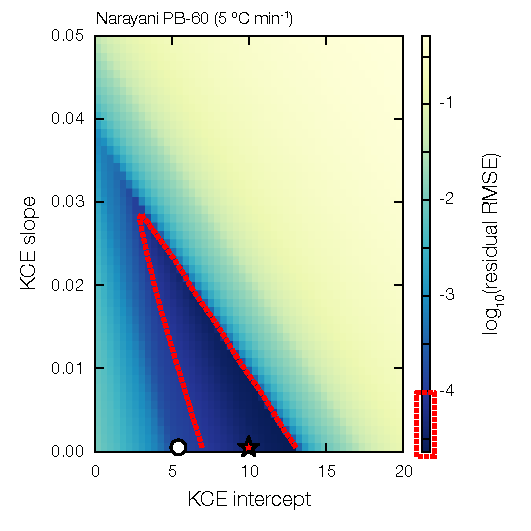
\includegraphics[]{Thesis_Figures/Ch3Fig5}}
	\caption[Residual RMSE using a range of KCE slopes and intercepts for Narayani PB-60]{Model residual RMSE using a range of KCE slopes and intercepts for Narayani PB-60 ($\beta$ = \SI{5}{\celsius.min^{-1}}). Each pixel represents the best-fit result using Equation \ref{Ch3Eq:20} for a given $k_{0}$ as determined by Equation \ref{Ch3Eq:21}. "Acceptable" fits with residual RMSE \num{\leq e-4} are contained within the red dotted line. Estimated result using the method of \citet{Miura:1998jf} for 3 ramp rates ($\beta$ = \SIlist{2;5;10}{\celsius.min^{-1}}) is plotted as a white circle, while the point corresponding to $k_{0}$ = \SI{e10}{\s^{-1}} (the value chosen for all samples in this study) is plotted as a red star.}
	\label{Ch3Fig:5} 
\end{figure}

\subsubsection{Tikhonov Regularization}

In principle, after choosing a value of $k_{0}$ and constructing the $\mathbf{A}$ matrix, the nonparametric pdf of $E$ that best describes an RPO thermogram can be determined using Equation \ref{Ch3Eq:20}. However, the inverse DAEM is highly sensitive to noise at the level of RPO instrument precision \citep[\textit{i.e.} approximately \SI{\pm 5}{ppm.\ce{CO2}}, \SI{\pm 5}{\celsius};][]{Hemingway:2016rc}, and is therefore ill-posed \citep{Hansen:1994uc}. To minimize this sensitivity to data uncertainty, we "smooth" the inverse DAEM solution using Tikhonov regularization \citep{Tikhonov:1977ui,Hansen:1994uc,Forney:2012dr,Forney:2012hz}. This approach is often used to solve constrained inverse problems by calculating an optimal solution that minimizes complexity in $p_{0}(E)$ (as determined by the intensity of fluctuations, or "roughness") while maximizing solution accuracy. Following \citet{Forney:2012hz}, we calculate roughness as the norm of the first derivative of $\mathbf{p}$:
%
% Equation 22
\begin{equation}\label{Ch3Eq:22}
	\left\| \frac{d p_{0}(E)}{dE} \right\| = \sqrt{ \sum_{l=1}^{n_{l}}\left( \frac{p_{l+1} - p_{l}}{E_{l+1} - E_{l}}\right)^{2}} = \| \mathbf{R} \cdot \mathbf{p} \| 
\end{equation}
%
where $\mathbf{R}$ is the discretized first derivative operator over the range of $E$ values considered. The regularized inverse solution can therefore be determined by including this roughness term when solving the constrained least squares:
%
% Equation 23
\begin{equation}\label{Ch3Eq:23}
	\min_{\mathbf{p}} \| \mathbf{A} \cdot \mathbf{p} - \mathbf{g} \|^{2} + \omega \| \mathbf{R} \cdot \mathbf{p} \|^{2}
\end{equation}
%
where $\omega$ is a scalar that determines how much to weight the roughness relative to the residual error. The best choice of $\omega$ is often considered to be the value that optimally minimizes the residual error and solution roughness. As described in \citet{Hansen:1994uc}, this is equal to the value corresponding to the point of maximum curvature in a $\log-\log$ plot of the residual error vs. the roughness when allowing $\omega$ to range over many orders of magnitude (\textit{i.e.} the so-called "L-curve", Figure \ref{Ch3Fig:6}). The best-fit $\omega$ value as determined by the L-curve therefore results in a "smoothed" solution of $p_{0}(E)$ with a residual error that is, in principle, approximately equal to the measurement uncertainty \citep{Forney:2012hz}. 

% Figure 6
\begin{figure}[p]
	\makebox[\textwidth][c]{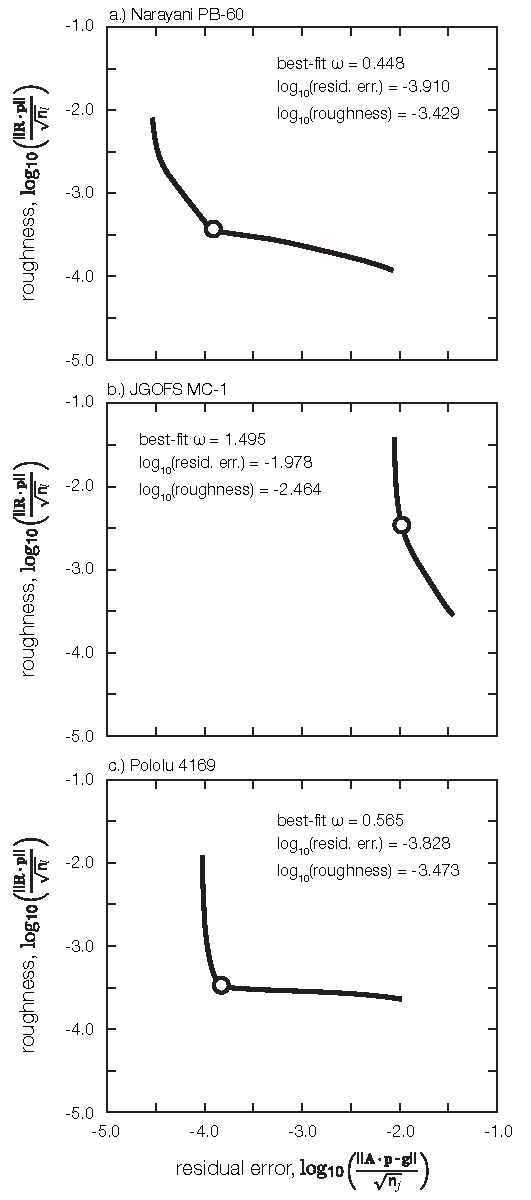
\includegraphics[]{Thesis_Figures/Ch3Fig6}}
	\caption[Tikhonov Regularization L-curves for all samples analyzed]{Tikhonov Regularization L-curves for all samples analyzed ($\beta$ = \SI{5}{\celsius.min^{-1}}): \textit{(A)} Narayani PB-60, \textit{(B)} JGOFS MC-1, and \textit{(C)} Pololu 4169. White circle corresponds to the point of maximum curvature -- \textit{i.e.} the best-fit $\omega$ value. Note the $\approx 100 \times$ higher residual error for JGOFS MC-1 due to the presence of carbonates.}
	\label{Ch3Fig:6} 
\end{figure}

However, we note that the best-fit residual error for JGOFS MC-1 is $\approx 100$-fold higher than for Narayani PB-60 and Pololu 4169 due to the non-first-order decay of \ce{CaCO3} that cannot be accurately predicted by the DAEM, as described above (Section \ref{Ch3Sec:3521}, Figure \ref{Ch3Fig:6}B). This results in a $G_{0}$-dependent $p_{0}(E)$ distribution, with the resulting $E$ value associated with the carbonate peak in this sample shifting from \SI{211}{kJ.mol^{-1}} when $G_{0}$ = \SI{98}{\micro g.C} to \SI{220}{kJ.mol^{-1}} when $G_{0}$ = \SI{951}{\micro g.C} (not shown). Still, regularized pdfs of $E$ for samples containing exclusively OC are nearly identical across all experimental conditions (\textit{i.e.} $\beta$, $G_{0}$), supporting the hypothesis that $p_{0}(E)$ is an intrinsic property of OC contained within a sample. For example, although there exist small differences between individual runs due to measurement uncertainty and variability in best-fit $\omega$ values (range of \numrange{0.044}{0.448}, $n=5$), the main features of the pdf of $E$ contained within Narayani PB-60 are robust for all conditions considered in this study (Figure \ref{Ch3Fig:7}). 

% Figure 7
\begin{figure}[t]
	\makebox[\textwidth][c]{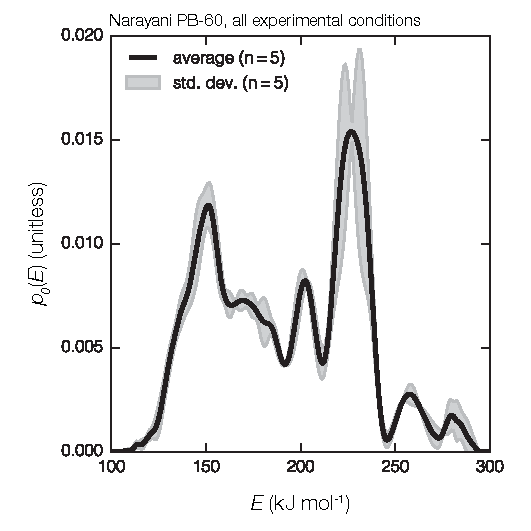
\includegraphics[]{Thesis_Figures/Ch3Fig7}}
	\caption[Average Narayani PB-60 $p_{0}(E)$ distribution for all experimental conditions]{Mean (black line) and standard deviation (gray shaded region) of regularized $p_{0}(E)$ distributions for Narayani PB-60 analyzed using a range of $G_{0}$ and $\beta$ values ($n = 5$), indicating that DAEM results are largely independent of experimental conditions for decarbonated samples.}
	\label{Ch3Fig:7} 
\end{figure}

Unlike previous studies that assume a Gaussian distribution of $p_{0}(E)$ during fossil fuel pyrolysis \citep{Lakshmanan:1994vs,Cai:2007hh,deCaprariis:2012jk}, regularized results calculated here clearly do not follow any parametric form (Figure \ref{Ch3Fig:8}, thick black lines). Rather, it can be seen that $p_{0}(E)$ generally resembles the RPO thermogram shape (Figure \ref{Ch3Fig:2}), as would be expected due to the fact that thermally recalcitrant OC is associated with higher values of $E$. Furthermore, observed high-frequency variability in $p_{0}(E)$ relative to the corresponding thermograms is an intrinsic result of non-isothermal kinetics. That is, during RPO analysis, OC associated with a single $E$ value will decompose over a range of temperatures with an increasing rate coefficient until it has been exhausted, thus resulting in a "smoothed" thermogram relative to the governing $p_{0}(E)$ distribution. Highly variable, non-parametric $p_{0}(E)$ observed here likely results from the extreme chemical complexity and  range of oxidation states contained in environmental OC samples \citep[\textit{e.g.}][]{Kellerman:2015jn}. In contrast, fossil fuel precursors have undergone various degrees of diagenesis and thermal maturation, potentially resulting in OC mixtures exhibiting more similar chemical properties that can be described by a Gaussian distribution of pyrolysis $E$ values \citep{Braun:1987vf}. This proposed relationship between $p_{0}(E)$ complexity and chemical diversity is additionally supported by the differences between samples analyzed herein. For example, fluvial suspended sediments such as Narayani PB-60 integrate a range of OC sources \citep[\textit{e.g.} recently fixed biomass, pre-aged soils, and eroded rock-derived material;][]{Blair:2012du} and would therefore be expected to contain a broader and more variable $p_{0}(E)$ distribution than that contained in a single soil OC sample such as Pololu 4169, as is observed (Table \ref{Ch3Tab:2}, \ref{Ch3Tab:4}; Figure \ref{Ch3Fig:8}A, \ref{Ch3Fig:8}C). We therefore propose that variability in the pdf of $E$ is a useful metric for comparing relative OC chemical complexity between samples.

% Figure 8
\begin{figure}[p]
	\makebox[\textwidth][c]{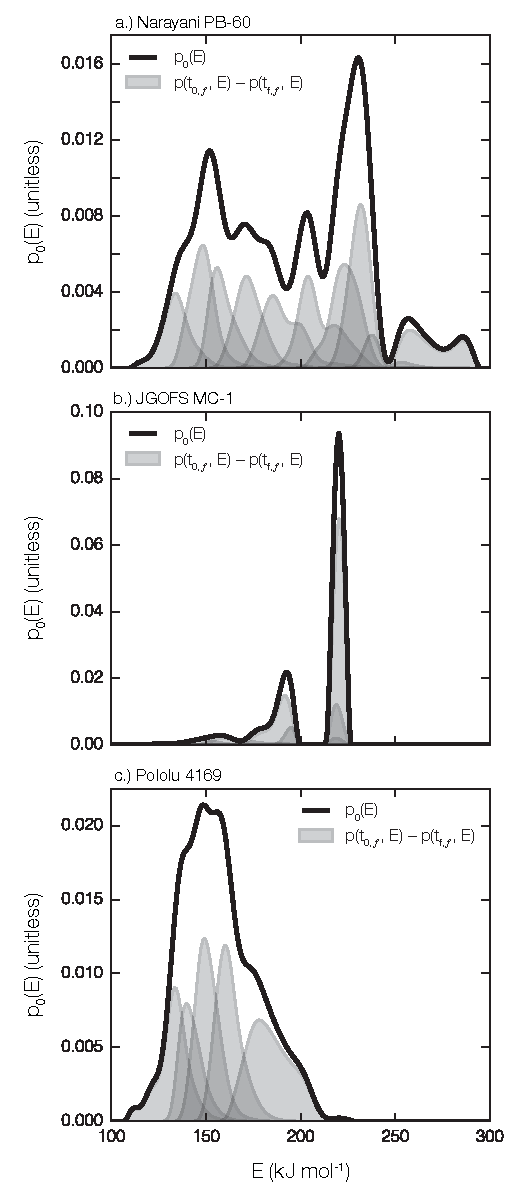
\includegraphics[]{Thesis_Figures/Ch3Fig8}}
	\caption[$p_{0}(E)$ distributions for all RPO fractions in all samples]{Regularized $p_{0}(E)$ distributions (black line) and the corresponding subset of $p_{0}(E)$ that is contained in each RPO fraction (gray shaded region): \textit{(A)} Narayani PB-60, \textit{(B)} JGOFS MC-1, and \textit{(C)} Pololu 4169. Overlapping distributions are a result of the fact that OC described by a single $E$ value decays over a range of temperatures.}
	\label{Ch3Fig:8} 
\end{figure}

\subsubsection{Determining $\bm{p_{0}(E)}$ contained in each RPO fraction}

To further understand how the distribution of OC molecular structure relates with source and reservoir age, we compare the average $E$ value corresponding to \ce{CO2} contained within each RPO fraction with its corresponding isotope composition. To do so, we first calculate the subset of the pdf of $E$ that is contained within an RPO fraction $f$ by taking the difference between $p(t,E)$ at the initial and final time points for each fraction. Because $A_{j,l}$ describes the relative amount of carbon initially associated with $E_{l}$ remaining at time $t_{j}$, it can be seen from Equation \ref{Ch3Eq:11} that the discretized $p(t_{j},E)$ values can be calculated by multiplying each $p_{l}$ in $\mathbf{p}$ by the corresponding element in the $j^{\text{th}}$ row of $\mathbf{A}$. The pdf of $E$ corresponding to the \ce{CO2} contained in each RPO fraction is therefore equal to $p(t_{\text{0},f},E) - p(t_{\text{f},f},E)$ for each value of $E$, where $t_{\text{0},f}$ and $t_{\text{f},f}$ are the initial and final time points, respectively, for RPO fraction $f$. Resulting distributions are typically non-parametric and highly overlapping, reflecting the fact that \ce{CO2} isotope composition for each RPO fraction is itself a weighted average of multiple sources (Figure \ref{Ch3Fig:8}, gray shaded regions). Average $E$ values and corresponding variance can thus be calculated as the first and second moments, respectively, of each distribution (Table \ref{Ch3Tab:2}--\ref{Ch3Tab:4}).

\subsection{Relationships between isotopes and reaction energetics}

\subsubsection{Kinetic isotope fractionation}

While not necessary for Fm because it is fractionation-corrected by definition \citep{Stuiver:1977uh,dosSantos:2007ca}, we must correct for any kinetic isotope effects occurring within the RPO instrument before interpreting \ce{\delta^{13}C} as a carbon source tracer \citep{Hemingway:2016rc}. If kinetic fractionation is large, as has been observed both during thermogenic methane formation \citep{Tang:2000ua,Cramer:2004tg} and dissolved OC oxidation by \textit{uv} light \citep{Oba:2008fv}, then this effect could overprint carbon source \ce{\delta^{13}C} signals. However, when directly measured using single-compound standards, \citet{Hemingway:2016rc} concluded that \ce{^{13}C} fractionation within the RPO instrument must be smaller than \SIrange{\approx 1}{\approx 2}{\permil}. Still, we correct the measured \ce{\delta^{13}C} values of each RPO fraction using the ratio of carbon-normalized \ce{^{13}C} and \ce{^{12}C} decomposition rates at each time point:
%
% Equation 24
\begin{equation}\label{Ch3Eq:24}
	\ce{^{13/12}r}(t) = \frac{\left( \frac{d \ce{^{13}}G(t)}{dt} \right)}{\left( \frac{d \ce{^{12}G}(t)}{dt} \right)} \left( \frac{\ce{^{12}G}_0}{\ce{^{13}G}_0} \right)
\end{equation}
%
Where we have added a preceding $12$ or $13$ superscript to specify isotope-specific variables. Following the Arrhenius equation, $\ce{^{13/12}r}(t)$ can be described as a function of the difference in $E$ between \ce{^{13}C}- and \ce{^{12}C}-containing molecules:
%
% Equation 25
\begin{equation}\label{Ch3Eq:25}
	\ce{^{13-12}\Delta E} = \ce{^{13}E} - \ce{^{12}E}
\end{equation}
%
Although \ce{^{13-12}\Delta E} is likely not identical for all compounds due to differences in the entropy and enthalpy of isotope substitution \citep{Tang:2000ua}, the estimated range of values for RPO analysis is small \citep[\SIrange{0.3e-3}{1.8e-3}{kJ.mol^{-1}};][]{Hemingway:2016rc}. We therefore assume \ce{^{13-12}\Delta E} = \SI{1.8e-3}{kJ.mol^{-1}} for all RPO fractions, noting that a choice of \SI{0.3e-3}{kJ.mol^{-1}} would result in \ce{\delta^{13}C} values that are identical to those calculated here within analytical uncertainty.

$\ce{^{13/12}r}(t)$ can be determined using the ratio of carbon-normalized, isotope-specific decay rates as calculated in Equation \ref{Ch3Eq:12} by substituting $p_{0}(\ce{^{12}E})$ and $p_{0}(\ce{^{13}E})$ for $p_{0}(E)$. Because carbon is present as \SI{\approx 99}{\%} \ce{^{12}C}, we set $p_{0}(\ce{^{12}E}) = p_{0}(E)$ such that $\frac{d \ce{^{12}G}(t)}{dt} = \frac{dG(t)}{dt}$. Corresponding $\frac{d \ce{^{13}G}(t)}{dt}$ can then be determined using $p_{0}(\ce{^{13}E}) = p_{0}(E + \ce{^{13-12}\Delta E})$. That is, \ce{^{13}C}-containing molecules decay at rates governed by a pdf of $E$ that is identical to $p_{0}(E)$ but has been shifted to the right by \SI{1.8e-3}{kJ.mol^{-1}}. We then correct the measured \ce{\delta^{13}C} values of each RPO fraction $f$ for kinetic isotope fractionation by dividing by the average $\ce{^{13/12}r}(t)$ value over the time of collection [written as $\mean{\ce{^{13/12}r}(t)_{f}}$]:
%
% Equation 26
\begin{equation}\label{Ch3Eq:26}
	\ce{\delta^{13}C}_{f, \text{corrected}} = \frac{1}{\mean{\ce{^{13/12}r}(t)_{f}}} \left( \ce{\delta^{13}C}_{f} + 1000 \left[ \mean{\ce{^{13/12}r}(t)_{f}} - 1 \right] \right)
\end{equation}
%
For the samples analyzed here,  $\ce{^{13/12}r}(t)$ is initially \num{\approx 0.999}, indicating slightly faster decay of \ce{^{12}C} at low temperatures, and gradually increases to \num{\approx 1.002} when $G(t) \ll 0.01 G_{0}$,  as has been described previously \citep{Cramer:2004tg,Hemingway:2016rc}. Resulting kinetic fractionation corrections are near or within analytical uncertainty, with absolute \ce{\delta^{13}C} values for all RPO fractions shifted by \SI{< 0.2}{\permil} ($\ce{\delta^{13}C}_{f, \text{corrected}} - \ce{\delta^{13}C}_{f}$: maximum = \SI{+0.16}{\permil}, Pololu 4169 fraction 1; minimum = \SI{-0.10}{\permil}, Narayani PB-60 fraction 9).

\subsubsection{Comparing $\bm{p_{0}(E)}$, \ce{^{13}C} content, and \ce{^{14}C} content}

In addition to exhibiting the narrowest and least complex pdf of $E$, Pololu 4169 displays a much smaller spread in both \ce{\delta^{13}C} and Fm values than does Narayani PB-60 (Figure \ref{Ch3Fig:9}A--D), supporting the idea that highly complex $p_{0}(E)$ distributions reflect the integration of multiple OC sources with variable chemical structures and reservoir ages. Pololu 4169 Fm values are low and stable for all RPO fractions (Figure \ref{Ch3Fig:9}B), indicating that low-$E$ OC can become significantly pre-aged given the proper environmental conditions \citep{Schmidt:2011gg}. Furthermore, Fm values for this sample display a small yet statistically significant increase with increasing $E$, opposite of what would be expected if thermal recalcitrance were a major driver of reservoir age (\SI{0.0001}{[kJ.mol^{-1}]^{-1}}, $R^{2} = 0.895$, $p$-value = \num{1.5e-2}). Coincident with increasing Fm, \ce{\delta^{13}C} decreases slightly with increasing $E$ (Figure \ref{Ch3Fig:9}A), suggesting a second source of \ce{^{13}C}-depleted, \ce{^{14}C}-enriched OC at higher $E$ values, potentially due to downward percolation of surface dissolved OC \citep{Chadwick:2007hc}. Still, the fact that Fm does not decrease with increasing $E$ is consistent with the current paradigm of soil carbon dynamics, which interprets reservoir age as an ecosystem property rather than a function of OC chemical structure \citep{Mikutta:2006gx,Janssens:2010hd,Schmidt:2011gg}. 

Pololu 4160 $p_{0}(E)$ distribution is concentrated at low $E$ values and is dominated by a large, broad peak despite the fact that soil OC contains a mixture of humic material, lipids, carbohydrates, lignin, \textit{etc.} \citep[Figure \ref{Ch3Fig:8}C;][]{Helfrich:2007ej}. RPO analysis therefore does not result in a separation of complex OC mixtures into individual, highly resolved peaks representing individual compounds or compound classes. Combined with a relatively homogenous \ce{\delta^{13}C} and Fm values between RPO fractions, a narrow $p_{0}(E)$ distribution indicates that individual compound classes contained in environmental samples are not separable based on thermal lability despite the unique decomposition temperatures when analyzed as purified compounds \citep{Williams:2014bq}. In contrast, it is well known that individual biomarkers such as lignin and \textit{n}-alkanoic acids contained in soils can display drastically different \ce{^{14}C} content \citep[see][for review]{Schmidt:2011gg}. The fact that this is not observed between RPO fractions is strong evidence that OC decomposing at any given $E$ value does not correspond to a single compound or simple set of compounds, but is rather derived from a mix of sources. This can be achieved, for example, if relatively oxidized functional groups decompose at low $E$ independent of their chemical source, while the remaining aromatic and aliphatic core structures resist degradation until higher temperatures have been reached. This interpretation indicates that RPO analysis separates OC based on the redox state and bonding environment of individual carbon atoms rather than properties of whole molecules, analogous to the process by which enzymes degrade OC in the environment \citep{Sinsabaugh:2008il}. 

% Figure 9
\begin{figure}[p]
	\makebox[\textwidth][c]{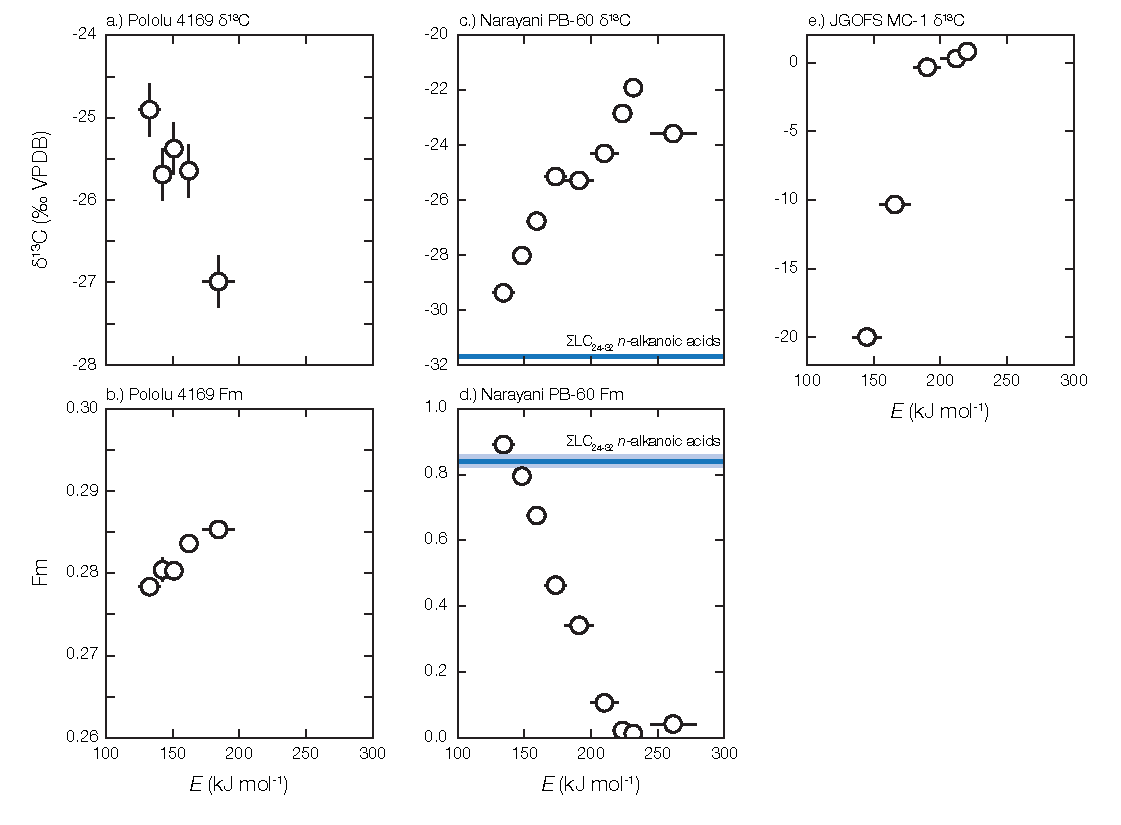
\includegraphics[]{Thesis_Figures/Ch3Fig9}}
	\caption[RPO $E$ vs. isotope plots for all fractions in all samples]{Plots of resulting $E$ vs. fractionation-corrected \ce{\delta^{13}C} or Fm for each sample analyzed: Pololu 4169 [\textit{(A)} \ce{\delta^{13}C}, \textit{(B)} Fm], Narayani PB-60 [\textit{(C)} \ce{\delta^{13}C}, \textit{(D)} Fm], and JGOFS MC-1 [\textit{(E)} \ce{\delta^{13}C}]. Error bars in \ce{\delta^{13}C} and Fm represent propagated analytical uncertainty, while error bars in $E$ are the standard deviation contained within each fraction. Blue lines in panel \textit{(C)} and \textit{(D)} are the $\Sigma$LC\sub{24--32} \textit{n}-alkanoic acid \ce{\delta^{13}C} and Fm values, with shaded regions representing the reported $\pm 1 \sigma$ uncertainty \citep{Galy:2011hk,Galy:2011ix}.}
	\label{Ch3Fig:9} 
\end{figure}

Still, significant trends in isotope composition with increasing $E$ can be observed. For example, the relationship between \ce{\delta^{13}C} and $E$ for Narayani PB-60 RPO fractions 1 through 8 is remarkably linear, with a slope of \SI{0.07}{\permil.(kJ.mol^{-1})^{-1}} ($R^{2} = 0.954$, $p$-value = \num{3.2e-5}; Figure \ref{Ch3Fig:9}C). The \SI{\approx 4}{\permil} \ce{^{13}C} depletion in fraction 9 relative to what would be expected based on this trend is at least partially due to charring, as has been described previously during non-isothermal OC pyrolysis \citep{Williams:2014bq}. Charring can result in an apparent shift toward higher $E$ values for labile OC compounds, as free-radical formation and subsequent condensation of aromatic material will increase thermal stability. However, because it has been shown that processes occurring in series can still be treated as a superposition of parallel reactions \citep{Forney:2014ws}, charring does not violate the kinetic model developed here. Rather, this simply results in a small inclusion of otherwise labile OC within the highest-temperature RPO fraction.

Nonetheless, fractions 1 through 8 strongly suggest that Narayani PB-60 OC contains 2 end members that mix linearly as a function of $E$. Importantly, although the isotope composition of \ce{CO2} contained in each RPO fraction represents a weighted average of OC associated with a particular $E$ range, this does not inherently require a linear mixing trend between fractions. For example, mixing two theoretical end members with identical $p_{0}(E)$ distributions but contrasting \ce{^{13}C} compositions will shift each RPO fraction along the \ce{\delta^{13}C} axis (\textit{i.e.} vertically in Figure \ref{Ch3Fig:9}C) according to the relative contribution of each end member, resulting in a "flat" \ce{\delta^{13}C} relationship with $E$. In contrast, a mixture of two end members containing drastically different chemical structures and thus non-overlapping $p_{0}(E)$ distributions would lead to two "clusters" of points in a plot of \ce{\delta^{13}C} vs. $E$. A linear trend like that observed here therefore indicates two end members with unique \ce{^{13}C} compositions yet complex, overlapping $p_{0}(E)$ distributions. That is, it requires a decrease in the contribution by a \ce{^{13}C}-depleted end member and a corresponding increase in the contribution by a \ce{^{13}C}-enriched end-member with increasing $E$. 

This is further evidenced by the similarly linear trend in Fm with increasing $E$ for RPO fractions 1 through 8 (slope = \SI{-0.01}{[kJ.mol^{-1}]^{-1}}, $R^{2} = 0.987$, $p$-value = \num{7.6e-7}). Unlike Pololu 4169, \SI{\approx 20 \pm 5}{\%} of OC contained in Narayani PB-60 is derived from the erosion of OC-rich bedrock in this catchment \citep[OC\sub{petro};][]{Galy:2008ff,Rosenheim:2012kh}. Because this material is \ce{^{14}C}-free by definition, and because it has been shown that similarly condensed "black" carbon pyrolyses above \SI{\approx 650}{\celsius} \citep{Williams:2014bq}, OC\sub{petro} is the likeliest source of high-$E$ OC in this sample. However, strong linear trends in both \ce{\delta^{13}C} and Fm with increasing $E$ require that a fraction of this material has been incorporated into lower $E$ OC, as the pyrolysis temperatures observed in \citet{Williams:2014bq} correspond to an $E$ value greater than \SI{\approx 200}{kJ.mol^{-1}}. Similar to the observation in Pololu 4169 that biospheric OC (OC\sub{bio}) generally contains low $E$ values, previously measured \ce{\delta^{13}C} and Fm values of long-chain \textit{n}-alkanoic acids extracted from Narayani PB-60 are consistent with the lowest $E$ RPO fractions \citep[Figure \ref{Ch3Fig:9}C--D;][]{Galy:2011hk,Galy:2011ix}. 

Therefore, a binary mixture combining biospheric OC\sub{bio} described by relatively homogenous Fm near that of \textit{n}-alkanoic acids and an $E$ distribution similar to Pololu 4169 with unaltered OC\sub{petro} described by $E \geq 200$ \si{kJ.mol^{-1}} would result in "clustered" RPO fractions in Figure \ref{Ch3Fig:9}D due to the lack of significant $E$ overlap. This is clearly not observed. Rather, the linear trends observed for both \ce{\delta^{13}C} vs. $E$ and Fm vs. $E$ require the presence of two end members with unique isotope compositions but overlapping $p_{0}(E)$. This further indicates that each "peak" in a distribution of $p_{0}(E)$ (\textit{e.g.} Figure \ref{Ch3Fig:8}A) does not represent an isotopically unique signal derived from a specific class of compounds. Instead, this implies that each end-member contains carbon atoms described by similar chemical bonding environments and redox states. RPO analysis is therefore ideally suited for separating isotopically unique yet chemically overlapping OC sources.

Lastly, we note that JGOFS MC-1 RPO \ce{\delta^{13}C} values are driven by a sharp increase in \ce{CaCO3} contribution at higher $E$ values, with fraction 5 matching the independently measured calcite value \citep[Figure \ref{Ch3Fig:9}E;][]{Sayles:2001ua}. Although carbon in this sample is present as \SI{\approx 95}{\%} calcite, the \ce{\delta^{13}C} value of fraction 1 is near that expected for phytoplankton biomass OC in this region \citep{Rau:1989wr}, suggesting that RPO analysis can sufficiently separate low-$E$ OC from \ce{CaCO3} despite the potential for catalysis, matrix effects, and non-first-order kinetics. Still, we emphasize that non-first-order kinetics and mass-dependent \ce{CaCO3} elution temperatures do hinder our ability to interpret changes in OC isotope composition for carbonate-containing samples. We therefore do not recommend quantitatively interpreting RPO isotope and $p_{0}(E)$ results from carbonate-rich samples without independent constraints on end-member composition. 

\section{Conclusion}

Serial oxidation techniques such as RPO are a promising new class of methods for relating OC chemical composition, isotopic composition, and environmental residence times. To better interpret these data, we develop an inverse kinetic model that determines the underlying distribution of activation energy required to thermally degrade OC. Unlike previous implementations of this model, our description does not require any \textit{a priori} assumptions about the shape of the pdf of $E$ values, $p_{0}(E)$, but rather determines the regularized non-parametric solution. By analyzing Narayani PB-60 using a range of oven ramp rates and initial masses, we show that the underlying $E$ distribution is independent of experimental conditions and is therefore an intrinsic property of the OC chemical bonding environment. In contrast, results from a \ce{CaCO3}-rich sample, JGOFS MC-1, indicate that inorganic carbon degradation rates cannot be predicted by our model, likely due to catalytic reactions and matrix effects during RPO analysis.

To compare reaction energetics with measured \ce{\delta^{13}C} and Fm values, we describe the temporal evolution of $p_{0}(E)$ during an RPO experiment and calculate the average $E$ value corresponding to the carbon contained in each fraction. After correcting \ce{\delta^{13}C} values for kinetic isotope fractionation, plots of \ce{\delta^{13}C} vs. $E$ and Fm vs. $E$ indicate that activation energy is strongly correlated with OC isotope composition for the samples analyzed herein. RPO results are consistent with hypothesized controls on OC source and residence time as determined by bulk and compound-specific isotope measurements. We therefore suggest that paired kinetic and isotopic measurements as determined by RPO analysis can offer novel insight into a range of carbon cycle processes.


%\section{Acknowledgements}

%We are grateful to the NOSAMS sample prep lab staff, especially Ann P. McNichol, Mary Lardie-Gaylord, and Alan Gagnon for assistance in running the RPO instrument and measuring isotope results. We thank Carl Johnson (WHOI) for bulk \%OC and \ce{\delta^{13}C} measurements and Katherine Grant (Cornell University) for supplying the RPO results for the Pololu 4169 sample. V.V.G. was partly supported by the US National Science Foundation (grants OCE-0851015 and OCE-0928582), the WHOI Coastal Ocean Institute (grant 27040213) and an Independent Study Award (grant 27005306) from WHOI; J.D.H. was partly supported by the NSF Graduate Research Fellowship Program under grant number 2012126152.

